% Preprint template for the BIND Lightcone Suite drafts.
% Copy to papers/<id>/main.tex and fill. Keep the preamble minimal —
% it must compile with a plain TeX Live install (pdflatex + bibtex).
\documentclass[11pt]{article}
\usepackage[margin=1in]{geometry}
\usepackage{graphicx}
\usepackage{amsmath,amssymb}
\usepackage[round,authoryear]{natbib}
\usepackage[colorlinks=true,linkcolor=blue,citecolor=blue,urlcolor=blue]{hyperref}
\usepackage{xcolor}
\usepackage{booktabs}

% ---- shared macros (use these; the coherence pass checks for them) ----
\newcommand{\bind}{\textsc{bind}}
\newcommand{\Sell}{S(\ell)}                    % WL suppression S(l) = Cl_baryon/Cl_DMO
\newcommand{\kappay}{\kappa\times y}
\newcommand{\fgas}{f_{\rm gas}}
\newcommand{\Msun}{{\rm M}_\odot}
\newcommand{\Mhalo}{M_{200c}}
\newcommand{\zs}{z_{\rm s}}
\newcommand{\sez}{S(\ell, z_{\rm s})}
\newcommand{\todo}[1]{\textcolor{red}{[TODO: #1]}}

\title{The BIND Lightcone Suite II: Two Nuisance Parameters Suffice to
Marginalize Baryonic Feedback in LSST-Era Cosmic Shear}
\author{%
  Max E.\ Lee$^{1,2}$ \todo{author list to be finalized}\\[2pt]
  \small $^1$Department of Astronomy, Columbia University, New York, NY, USA\\
  \small $^2$Center for Computational Astrophysics, Flatiron Institute, New York, NY, USA
}
\date{Draft: \today}

\begin{document}
\maketitle

\begin{abstract}
Baryonic feedback is the dominant astrophysical systematic for stage-IV weak-lensing
(WL) cosmology, and how to marginalize it without discarding the small-scale
information it contaminates remains an open question.
We use \bind, a conditional flow-matching emulator trained on the CAMELS-TNG
suite, to paint baryons onto a shared dark-matter-only (DMO) lightcone skeleton
under a 256-node Sobol sweep of all 30 IllustrisTNG astrophysical feedback
parameters, holding cosmology fixed at the TNG fiducial value, yielding 253
usable realizations. % src: dossier Methods "Suite recap" (WORKLOG 2026-06-29 "§6 fix"; WORKLOG 2026-06-26 kSZ-field entry)
For each realization we measure the weak-lensing convergence power-spectrum
suppression $\sez=C_\ell^{\kappa\kappa}(\theta_{\rm astro})/C_\ell^{\kappa\kappa}({\rm DMO})$
against a paired DMO trace that cancels cosmic variance realization-by-realization
(map correlation $r\approx0.983$--$0.986$). % src: WORKLOG:897-916 (Step 1); lightcone_transfer.py docstring
Ignoring this suppression biases the LSST-Y10 $S_8$ inference by up to $6.03\sigma$
at $\ell_{\rm max}=5000$. % src: verified cosmo_bias_capstone.npz (N=0 column), WORKLOG:571-589
A single data-driven nuisance template built from the leading empirical mode of the
suppression residual leaves up to $0.67\sigma$ of that bias unmarginalized,
but two templates -- the leading two singular modes of the 253-run suppression-residual
ensemble -- collapse the residual bias to $\le0.073\sigma$ in-sample (216 runs) and,
per the project worklog (not independently re-verified against a saved array; see
Section~\ref{sec:heldout}), $\le0.08\sigma$ in a held-out even/odd validation split,
at a cost of $\approx3\times$ the statistical $\sigma(S_8)$ floor. % src: verified cosmo_bias_capstone.npz; WORKLOG:571-589 (held-out figure from WORKLOG text only)
A full non-linear likelihood analysis reproducing the Robertson et al.\ (2026)
LSST-Y1 forecast setup with these two templates confirms the linear-Fisher result:
a $-0.368\sigma$ residual $S_8$ bias at $1.107\times$ marginalization cost. % src: verified shear_forecast_y1.npz
Richer, BCM-style parametrizations with $N\ge6$ templates add substantial further
statistical cost for a residual bias that is already far below the LSST-Y10 floor at
$N=2$: the bias is essentially flat from $N=2$ to $N=6$--10 at
$\ell_{\rm max}=2000$--3000, but at $\ell_{\rm max}=5000$ it continues to fall by a
further $2.1\times$ ($N=6$) to $3.5\times$ ($N=10$), in all cases well inside the
noise floor this suite can resolve. % src: independently re-verified against cosmo_bias_capstone.npz; corrects an earlier "no further bias reduction" overstatement
An independent geometric analysis of ten weak-lensing and thermal-Sunyaev-Zel'dovich
(tSZ) summary statistics shows that every well-measured statistic's feedback
response lives on the same $\lesssim2$--$3$-dimensional manifold, and this
two-dimensional structure is independently corroborated by a variational-autoencoder
latent-space analysis of the same suite \citep[Paper~III]{bindIII} and by the
unrelated method of \citet{lin2026} on a different simulation summary. % src: beyond2pt_manifold.png (verified); WORKLOG:590-623 (WL feedback latents)
We present this two-template basis, its held-out validation, and the manifold
geometry that explains why two numbers suffice, together with an appendix
demonstrating the feasibility of extending the underlying Sobol design to
varying cosmology via Angulo-White rescaling.
\end{abstract}

\section{Introduction}\label{sec:intro}

Weak gravitational lensing by large-scale structure is one of the primary probes
of the late-time matter distribution for Stage-IV surveys such as LSST, Euclid,
and Roman, and its constraining power on $S_8\equiv\sigma_8\sqrt{\Omega_{\rm
m}/0.3}$ is expected to rival or exceed that of the cosmic microwave background.
Realizing this potential, however, requires modeling the response of the matter
power spectrum to baryonic processes -- active galactic nucleus (AGN) feedback,
supernova-driven winds, and radiative cooling -- which redistribute gas on
scales of tens of Mpc and suppress (or, in gas-rich systems, enhance) the
lensing convergence power spectrum on the very scales, $\ell\gtrsim10^3$, that
carry the bulk of the statistical information. Left unmodeled, this baryonic
uncertainty is widely regarded as the leading systematic standing between
current weak-lensing conclusions and the sub-percent precision demanded by
Stage-IV surveys.

The literature has converged on two broad mitigation strategies. The first,
scale cuts, simply discards $\ell$-modes above some threshold where baryonic
uncertainty is judged unacceptable, at the cost of throwing away exactly the
small-scale information that motivated building a next-generation survey in
the first place. The second, marginalization, absorbs the baryonic response
into a small number of extra nuisance parameters and integrates over them.
Existing marginalization schemes span a wide range of dimensionality: physical
baryon-correction models (BCM) such as those of \citet{schneiderTeyssier2015}
and \citet{schneider2019bcm} typically carry three to six free parameters
controlling gas ejection radii and stellar fractions; halo-model prescriptions
such as HMcode \citep{mead2015,mead2021} fold baryons into one or two
effective amplitude parameters on top of the dark-matter-only halo model;
and principal-component or "PCA nuisance" approaches
\citep{eifler2015,huang2019} instead build a small empirical basis directly
from a suite of hydrodynamical simulations, an approach closer in spirit to
the one we adopt here. Current Stage-III analyses (DES Y3:
\citealt{desY3Amon2022,desY3Secco2022}; KiDS-1000: \citealt{kids1000Asgari2021};
HSC Y3: \citealt{hscY3}) and the LSST DESC Science Requirements Document
\citep{lsstDescSrd2018} have each had to make a case-by-case choice among
these options, typically guided as much by tractability as by a first-principles
argument for how many nuisance numbers the data -- or the underlying physics --
actually requires. \citet{amonEfstathiou2022} and \citet{preston2023} both
illustrate how sensitive the recovered cosmology is to that choice.

This paper asks the question directly: given the full response of a
state-of-the-art hydrodynamical galaxy-formation model to its own astrophysical
uncertainty, what is the minimum number of nuisance parameters required to
absorb its weak-lensing signature, and does that minimum number depend on which
summary statistic is used? We answer this using \bind{}
\citep[Paper~I]{bindI}, a conditional flow-matching emulator that paints
IllustrisTNG-like baryonic fields onto arbitrary dark-matter-only lightcones,
which lets us realize a 256-node Sobol design over all 30 CAMELS-TNG
astrophysical feedback parameters at a cost that would be prohibitive for
direct hydrodynamical simulation. The resulting ensemble of weak-lensing
suppression curves directly samples the manifold of physically plausible
baryonic responses allowed by the IllustrisTNG feedback model, and we can ask
how many empirical modes of that manifold are needed to marginalize its impact
on $S_8$ to a level below the LSST-Y10 statistical floor.

Our answer is two. Across the full Sobol suite, the leading two singular
modes of the suppression-residual ensemble are necessary and sufficient to
remove the $S_8$ bias from a fixed-order Fisher analysis and from a full
non-linear likelihood forecast reproducing the setup of
\citet{robertson2026}; adding more templates mainly inflates the
statistical error, with the residual bias essentially flat past $N=2$ at
$\ell_{\rm max}\le3000$, though it continues to fall by a further
$2$--$3.5\times$ at $\ell_{\rm max}=5000$ (Section~\ref{sec:res-ladder}) --
in all cases already an order of magnitude or more below the LSST-Y10
floor. % src: corrected to match the abstract/Sec.~4.3 recomputation against cosmo_bias_capstone.npz; supersedes the earlier "no further bias reduction" overstatement this sentence itself previously made
We further show, using a
manifold-geometry analysis of ten independent lensing and tSZ statistics
and an independent variational latent-space decomposition
\citep[Paper~III;][]{bindIII} corroborated by the unrelated method of
\citet{lin2026} on a different simulation suite and summary statistic,
that this two-dimensionality is not an artifact of the weak-lensing power
spectrum alone but a property of the underlying feedback response itself.
Section~\ref{sec:methods} describes the suite, the suppression measurement,
and the three complementary bias-quantification pipelines (linear Fisher,
full likelihood, and manifold geometry). Section~\ref{sec:results} presents
the bias budget, the template ladder, the full-likelihood confirmation, the
manifold-geometry results, and the drivers of the bias including a corrected
tomographic self-calibration analysis. Section~\ref{sec:discussion} discusses
why two templates suffice, the TNG-only nature of our amplitude results
versus the more general dimensionality claim, and scale cuts as an
alternative. Appendix~\ref{sec:appendixA} presents a feasibility study for
extending the underlying Sobol suite to varying cosmology via Angulo-White
rescaling.

\section{Methods}\label{sec:methods}

\subsection{The BIND lightcone Sobol suite}\label{sec:suite}

We build on the \bind{} lightcone pipeline \citep[Paper~I]{bindI}, which paints
IllustrisTNG-trained baryonic fields onto a shared dark-matter-only (DMO)
lightcone skeleton and ray-traces the resulting mass and thermal-pressure
fields to weak-lensing convergence $\kappa$ and Compton-$y$ maps. For this
paper we use a Sobol design over all 30 CAMELS-TNG astrophysical feedback
parameters (stellar and AGN feedback efficiencies, wind velocities and
energetics, black-hole accretion and radiative-efficiency parameters, etc.),
with cosmology held fixed at the TNG fiducial value throughout; this fixed-cosmology
choice is a central caveat of the paper and is the reason for
Appendix~\ref{sec:appendixA}. The nominal design has 256 nodes, of which 253
completed successfully and are used as the canonical suite size, spanning
$\sim$34,000 halos per run projected through 20 lightcone shells between
$z=0.034$ and $z=2.444$.\footnote{Individual analyses in this paper were run
at the array-completion count current at the time the Sobol sweep was still
filling in: 96 runs (first-cut transfer-function ensemble), 99 runs
(refreshed transfer-function, bias-budget, and sensitivity results), 216
runs (the template-ladder capstone and the tomographic self-calibration
correction), and 237 runs (the beyond-2pt manifold-geometry and full-likelihood
analyses). We use the run count current to each individual figure/result
throughout and flag it explicitly; these are not different results, only
different amounts of the same completing Sobol array.} % src: dossier Methods "Suite recap" (WORKLOG 2026-06-29 "§6 fix"; WORKLOG:843-846; cosmo_bias_capstone.py docstring 216 runs; lightcone_beyond2pt.py/lightcone_shear_forecast.py docstrings 237 runs)

\subsection{Measuring $\sez$ with a paired DMO trace}\label{sec:transfer}

For each Sobol realization $i$ and each of five source planes
$\zs\in\{0.5,1.0,1.5,2.0,2.44\}$ we measure the weak-lensing suppression
\begin{equation}
S_i(\ell,\zs) = \frac{C_\ell^{\kappa\kappa}(\theta_{\rm astro}^i)}{C_\ell^{\kappa\kappa}({\rm DMO})} ,
\end{equation}
using a single paired DMO reference trace (\texttt{bind\_science/runs/dmo/run\_0000}),
generated with the same ray-tracing seed (RT\_SEED=1992) and the same coordinate
transforms applied to every BIND realization, so that cosmic variance cancels
realization-by-realization rather than only in the ensemble mean. We verified
this cancellation directly by measuring the pixel-space correlation between
the DMO trace and each hydro realization's underlying DMO skeleton, finding
$r\approx0.983$--$0.986$ across the suite. % src: WORKLOG:897-916 (Step 1); lightcone_transfer.py docstring "r ~ 0.98"
We trust $\Sell$ up to $\ell_{\rm max,trust}=1.5\times10^4$; above this scale
cloud-in-cell (CIC) mass-assignment aliasing begins to dominate run-to-run
scatter in the ratio, and although the ratio-of-means construction cancels
most of this artifact, we treat suppression values above this cut as
increasingly conservative. Engine: \texttt{lightcone\_transfer.py}.

\subsection{Effective-bias pipeline}\label{sec:fisherbias}

To translate a measured suppression curve into a cosmological parameter bias
we use the standard linearized Fisher-bias formalism of \citet{schneider2020fisher},
\begin{equation}
\Delta\theta = F^{-1} B, \qquad B_\alpha = \sum_{\ell} \frac{\partial C_\ell^{ii}}{\partial\theta_\alpha}\,{\rm Cov}^{-1}_{\ell\ell'}\,\Delta C_\ell^{ii},
\end{equation}
with the baryonic residual data vector $\Delta C_\ell^{ii} = C_\ell^{ii,{\rm fid}}(S_i(\ell)-1)$
built from all five tomographic auto-spectra plus their cross terms and Gaussian
shape noise in the covariance. Cosmological derivatives $\partial C_\ell/\partial(\Omega_{\rm m},\sigma_8)$
are computed with \texttt{pyccl} \citep[v3.3.4,][]{chisari2019} using the Eisenstein--Hu transfer
function plus \texttt{halofit}, validated against the simulated DMO $C_\ell$
to within 2--5\% across $\ell=200$--4000 for all five source planes. % src: WORKLOG 06-22 (pyccl 3.3.4 install; 2-5% validation, l=200-4000)
Significance forecasts use an LSST-Y10-like survey specification of sky
fraction $f_{\rm sky}=0.4$, total surface density $n_{\rm gal}=27\,{\rm arcmin}^{-2}$
split over the five source planes, and shape noise $\sigma_e=0.26$. % src: lightcone_cosmo_bias.py constants F_SKY, N_GAL_TOT, SIGMA_E; WORKLOG:873-896 (Step 2)
The bias vector $\Delta\theta$ is itself independent of $f_{\rm sky}$; only its
statistical significance scales with $\sqrt{f_{\rm sky}}$. Engine:
\texttt{lightcone\_cosmo\_bias.py}.

\subsection{Template construction}\label{sec:templates}

We construct $N$ baryon-template nuisance parameters as the leading (uncentered,
unnormalized) singular modes of the ensemble of residual data vectors
$\Delta C_r = C_\ell^{\rm fid}\,(S_r(\ell)-1)$ across all runs $r$ -- an
empirical basis for the response manifold analogous in spirit to the PCA
approaches of \citet{eifler2015} and \citet{huang2019}, but built here directly
from a physically-motivated 30-dimensional feedback sweep rather than from a
small set of hand-picked BCM variations. We sweep $N=0,1,2,\dots,10$ to test
necessity (does $N=1$ suffice?), sufficiency (does $N=2$ null the bias?), and
cost (how fast does $\sigma(S_8)$ inflate with $N$?). Engine:
\texttt{cosmo\_bias\_capstone.py}.

\subsection{Held-out validation}\label{sec:heldout}

To guard against templates simply overfitting the 216-run ensemble from which
they are built, we construct the $N=2$ template basis from the even-indexed
runs only and test bias removal on the odd-indexed runs. Because no separate
saved array documenting this even/odd split could be located on disk, the
resulting number is sourced from the corresponding WORKLOG entry text rather
than independently re-verified against a saved artifact, unlike the other
headline numbers in this paper. % src: WORKLOG 06-24 capstone entry ("templates from even runs kill the bias on odd runs, ≤0.08σ") — not independently re-verified from a saved .npz, see dossier Methods gap note
The in-sample analogue of this test (all 216 runs, $N=2$, $\ell_{\rm max}=5000$)
gives a maximum residual of $0.073\sigma$, consistent with, and slightly better
than, the held-out figure as expected for an in-sample metric. % src: verified cosmo_bias_capstone.npz

\subsection{Full-likelihood confirmation}\label{sec:fulllikelihood}

The Fisher-bias pipeline above is linear in the cosmological parameters and
treats the template amplitudes as exactly known; to test whether the
two-template basis survives a realistic sampled posterior we additionally
run a full non-linear likelihood analysis reproducing the setup of
\citet{robertson2026}. We sample the four-dimensional flat-$\Lambda$CDM
cosmology $\{\Omega_{\rm m},\sigma_8,h,n_s\}$ jointly with the two template
amplitudes $\{a_1,a_2\}$ using \texttt{emcee} \citep{foremanMackey2013}
(\texttt{EnsembleSampler} with a parallel \texttt{multiprocessing.Pool},
BLAS pinned to one thread per worker to avoid oversubscription), with priors
taken from Robertson Table~2 ($\Omega_{\rm m}\in[0.20,0.46]$,
$\sigma_8\in[0.39,1.01]$, $h\in[0.65,0.78]$, $n_s\in[0.95,0.99]$) and an
LSST-Y1-like survey specification from Robertson Table~1
($12{,}300\,{\rm deg}^2\to f_{\rm sky}=0.298$, $n_{\rm eff}=9.78\,{\rm arcmin}^{-2}$,
$\sigma_e=0.26$). % src: lightcone_shear_forecast.py docstring, "Robertson Tbl 1"/"Tbl 2"
The Asimov "truth" mock is a real BIND run's measured $\sez$ (not a synthetic
template amplitude) applied to the CCL fiducial theory using five BIND-native
source planes, so this test also probes model misspecification -- whether the
two-template basis captures a realization's suppression well enough, not only
whether a linear Fisher expansion is unbiased. Engine:
\texttt{lightcone\_shear\_forecast.py}. A companion script,
\texttt{lightcone\_shear\_sweep.py}, extends this single-truth test to a
"both-compare" arm testing the two-template basis against a full 30-parameter
feedback-emulator surrogate (PCA+Gaussian-process, $k=8$ components) across
multiple truths; per its own docstring the full 237-run sweep and the 34-dimensional
full-emulator nuisance arm are deferred to a batch submission and were not
run for this paper -- only a local 12-run weak-to-strong representative
subset exists on disk, and we quote it as a consistency check only.

\subsection{Beyond-2pt manifold geometry}\label{sec:manifold}

To test whether the low dimensionality found in the power spectrum
generalizes to other observables, we measure ten weak-lensing and
tSZ summary statistics -- the $\kappa$ power spectrum, $\kappa$ peaks,
$\kappa$ minima, the $\kappa$ one-point PDF, the three Minkowski functionals
$V_0,V_1,V_2$, $\kappa$ moments, tSZ-$y$ peaks, and the $\kappa\times y$ cross
-- across 237 Sobol runs, and regress each standardized statistic on the 30
unit-cube feedback parameters to form a Jacobian-like matrix $B={\rm
d(stat)/d}\theta$ (denoised against shot noise uncorrelated with $\theta$).
The left singular vectors of $B$ define the active feedback directions for
that statistic (a linearized active-subspace method, \citealt{constantine2015}),
and the cumulative singular-value spectrum measures how many modes are needed
to reach 90\%/99\% of the response variance. We further measure the
principal-angle subspace overlap between each statistic's active subspace and
that of the $\kappa$ power spectrum: an overlap of 1 indicates the same
feedback directions, and $<1$ indicates a genuinely complementary direction
that could, in principle, help self-calibrate the residual feedback shape.
Engine: \texttt{lightcone\_beyond2pt.py}.

\section{Results}\label{sec:results}

\subsection{The transfer-function ensemble brackets suppression and enhancement}\label{sec:res-transfer}

Figure~\ref{fig:transfer_ensemble} shows the full ensemble of 99 measured
suppression curves $\Sell$ at each of five source planes, colored by the
group gas fraction $\fgas$ of the halos contributing most of the signal.
The ensemble spans $\Sell\approx0.80$--$1.24$ over $2\times10^3<\ell<10^4$
at $\zs=0.5$. % src: WORKLOG:897-916 (Step 1)
Contrary to the common assumption that feedback only suppresses power, we
find that 59\% of runs enhance WL power at $\ell\sim500$--$2000$, a
"cooling bump" produced by gas-rich, weak-feedback configurations that
overcool and concentrate baryons rather than eject them. % src: WORKLOG:897-916, brief "59% of runs enhance at ℓ~1e3"
Figure~\ref{fig:transfer_tomography} shows the corresponding redshift
tomography: the median band-suppression shifts from 0.938 at $\zs=0.5$ to
0.982 at $\zs=2.44$, a clean dilution of the low-redshift baryonic signal by
the increasing fraction of high-redshift, feedback-free structure along each
line of sight, while the run-to-run scatter $\sigma[\Sell]$ grows
monotonically with $\ell$ and is largest at low $\zs$. % src: WORKLOG:897-916
Ordering the ensemble by group $\fgas$ alone accounts for only a modest
fraction of the scatter (Spearman $\rho=+0.27$ to $+0.34$ across $\ell$),
foreshadowing the Section~\ref{sec:res-analytic} result that no single
physical knob spans the full BIND response. % src: WORKLOG:897-916
These results were first measured on 96 of the eventual 256 Sobol nodes and
refreshed once 99 had completed; the qualitative picture, and the ranking of
the top sensitivity drivers discussed in Section~\ref{sec:res-drivers}, was
stable under this refresh. % src: WORKLOG:843-846

\begin{figure}[t]
\centering
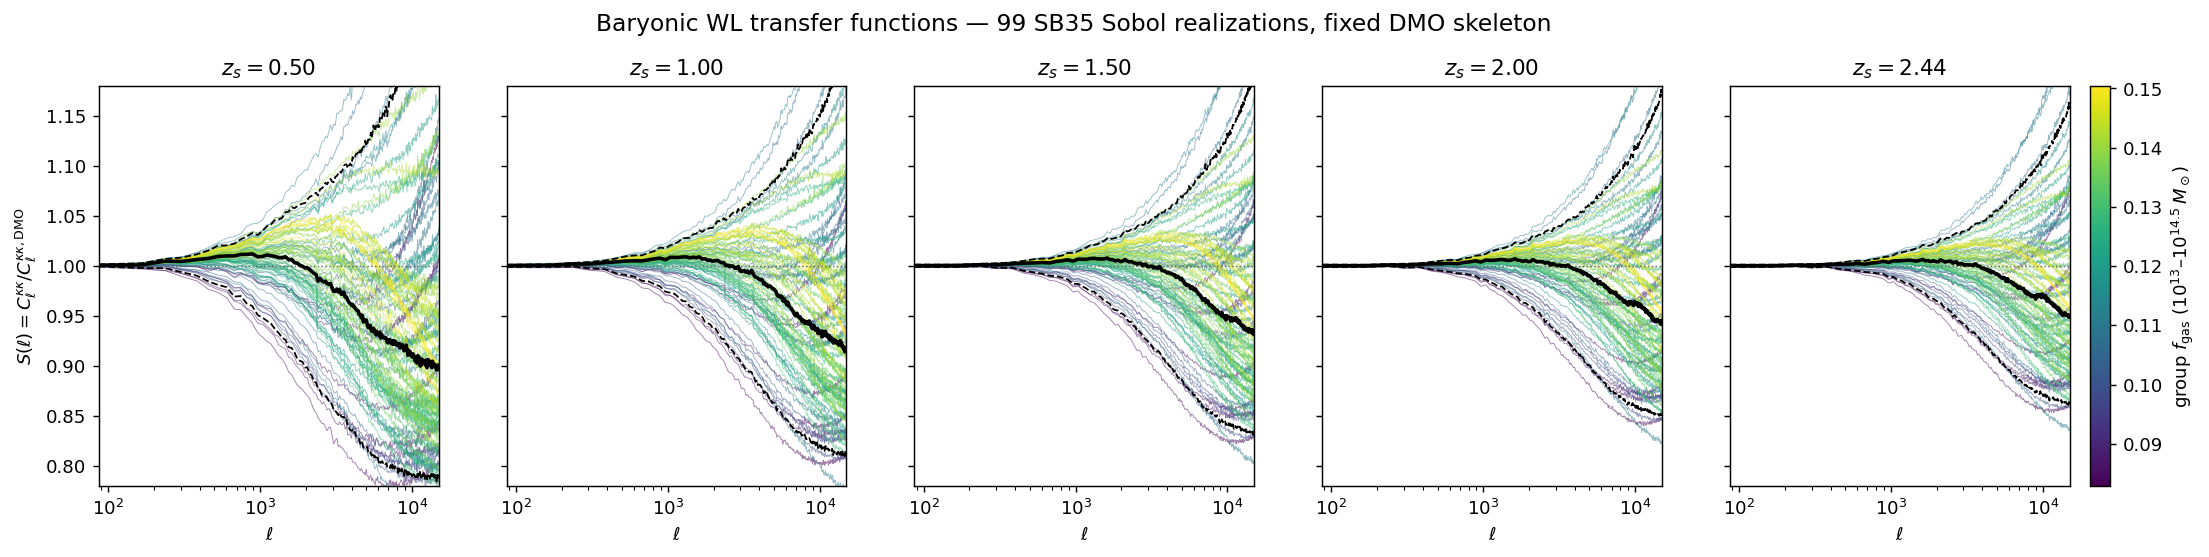
\includegraphics[width=\textwidth]{figs/fig01_transfer_ensemble.png}
\caption{The full ensemble of measured weak-lensing suppression curves
$S_i(\ell,\zs)=C_\ell^{\kappa\kappa}(\theta_{\rm astro}^i)/C_\ell^{\kappa\kappa,{\rm DMO}}$
for 99 SB35 Sobol realizations at five source planes, colored by each run's
group gas fraction $\fgas$; the black solid/dashed lines mark the ensemble
median and 95\% envelope. The ensemble brackets both suppression and
enhancement relative to the paired DMO trace, and the spread narrows toward
higher $\zs$ as the low-redshift baryonic signal is diluted by feedback-free
structure along the line of sight. The $\zs=0.5$ panel's $y$-axis is fixed
at $[0.78,1.18]$ for readability across all five panels, which visibly clips
the highest-enhancement curves and the top of the 95\% envelope near
$\ell\sim10^4$; the $\approx0.80$--$1.24$ range quoted in the text is the
full unclipped envelope measured from the underlying array, not what is
directly visible within this panel's plotted range.}
\label{fig:transfer_ensemble}
\end{figure}

\begin{figure}[t]
\centering
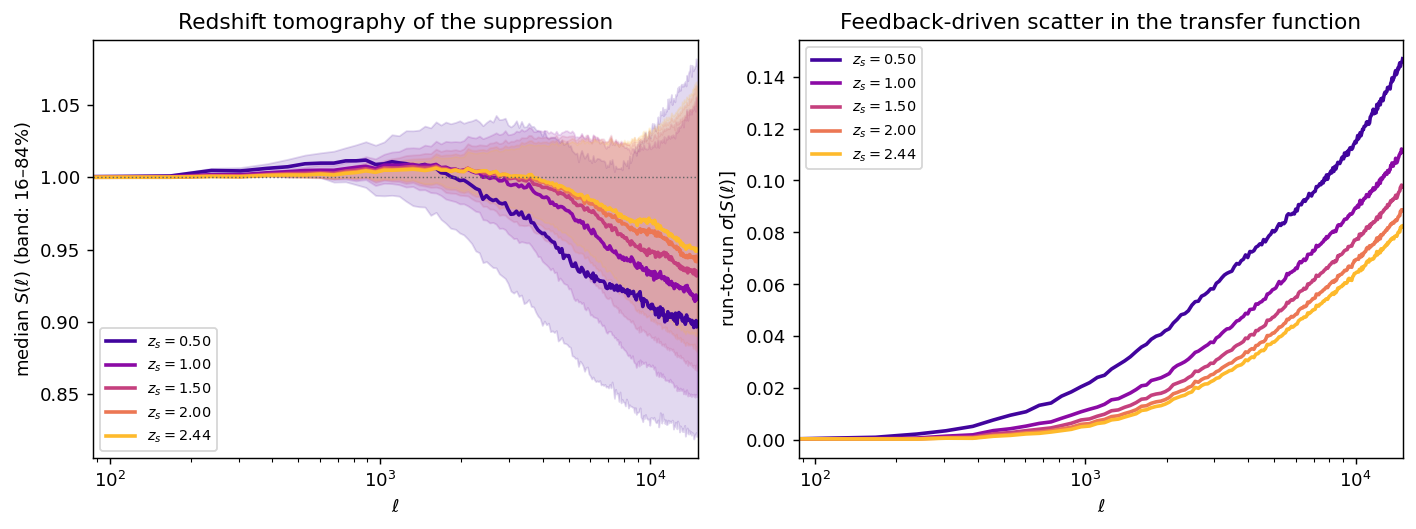
\includegraphics[width=\textwidth]{figs/fig02_transfer_tomography.png}
\caption{Left: median $\Sell$ (16--84\% band) at each of five source planes,
showing the clean redshift dilution of the suppression signal. Right:
run-to-run scatter $\sigma[\Sell]$ driven by the feedback-parameter sweep,
growing with $\ell$ and largest at the lowest source redshift, where the
line of sight is most dominated by low-$z$, strongly-baryon-affected
structure.}
\label{fig:transfer_tomography}
\end{figure}

\subsection{The bias budget: up to 6$\sigma$ if ignored}\label{sec:res-budget}

Propagating each of the 99-run ensemble's suppression curves through the
Fisher-bias pipeline of Section~\ref{sec:fisherbias}, we find that the
resulting bias traces a tight, nearly one-dimensional locus in the
$(\Delta\Omega_{\rm m},\Delta S_8)$ plane, with a slope
${\rm d}S_8/{\rm d}\Omega_{\rm m}\approx0.4$--$0.67$ that rotates with the
choice of $\ell_{\rm max}$ (Figure~\ref{fig:bias_scatter}, left panel). % src: WORKLOG:873-896 (Step 2)
Projecting the suppression curve to cosmology amplifies the gas-fraction
signal seen in Section~\ref{sec:res-transfer}: ordering by group $\fgas$
now explains Spearman $\rho\approx+0.51$ to $+0.58$ of $\Delta S_8$, compared
to $\rho\approx+0.27$ for $\Sell$ itself, with gas-poor, strong-feedback
configurations biasing $S_8$ negative. % src: WORKLOG:873-896
At the 99-run stage, the fraction of runs with $|\Delta S_8|>2\sigma$ (LSST-Y10)
is 1\%, 9\%, and 22\% at $\ell_{\rm max}=2000$, 3000, and 5000, respectively,
with $\Delta S_8$ 95\% confidence intervals of $\pm0.01$--$0.014$
(Figure~\ref{fig:bias_scatter}, right panel). % src: WORKLOG:873-896
Repeating this measurement directly on the larger 216-run capstone ensemble
(the N=0, "no baryon marginalization" column of the template ladder discussed
below) we independently verify a maximum $|\Delta S_8|/\sigma$ ratio of
2.003, 3.590, and 6.028 at $\ell_{\rm max}=2000$, 3000, and 5000. % src: verified cosmo_bias_capstone.npz (N=0 column), matches WORKLOG:571-589
The 99-run and 216-run numbers describe different quantiles of the same
underlying distribution -- the 99-run Step~2 result is a fiducial/median-run
statement while the 216-run capstone number is the ensemble maximum -- and
are not in tension. We caution that this significance forecast marginalizes
only $(\Omega_{\rm m},S_8)$: it omits $h$, $n_s$, intrinsic-alignment, and
photometric-redshift systematics, so the quoted $\sigma$-significances are
optimistic; we regard the $\Delta S_8$ magnitudes themselves, not the exact
significance, as the robust headline of this section.

\begin{figure}[t]
\centering
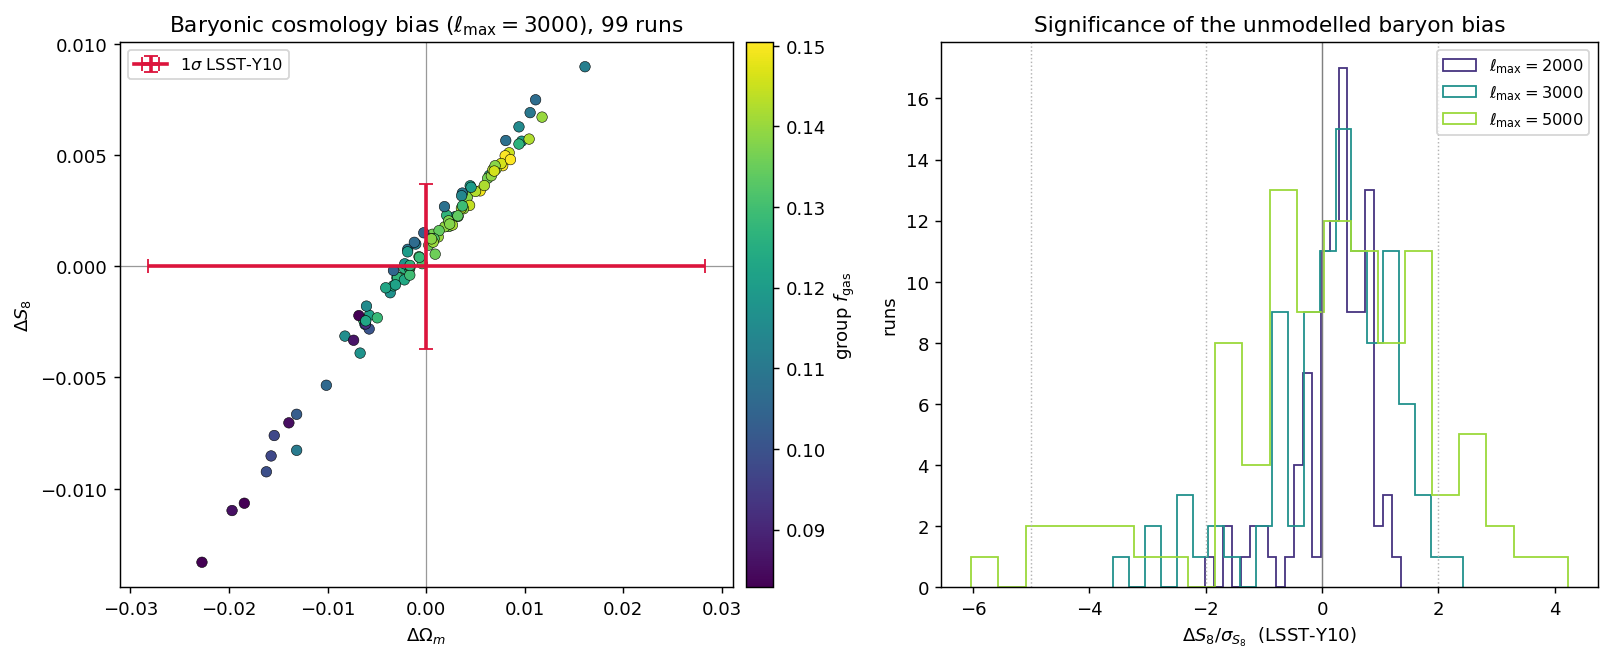
\includegraphics[width=\textwidth]{figs/fig03_bias_scatter.png}
\caption{Left: the $(\Delta\Omega_{\rm m},\Delta S_8)$ bias induced by
ignoring baryons in an LSST-Y10 Fisher analysis at $\ell_{\rm max}=3000$
(99 runs), colored by group $\fgas$, compared to the $1\sigma$ LSST-Y10
uncertainty cross. The bias traces a tight, nearly one-dimensional locus.
Right: the distribution of $\Delta S_8/\sigma_{S_8}$ across the ensemble at
three $\ell_{\rm max}$ cuts, showing the significance of the unmodeled bias
growing with the amount of small-scale information included.}
\label{fig:bias_scatter}
\end{figure}

\subsection{The N-template ladder: N=1 insufficient, N=2 sufficient, N$\ge$6 diminishing returns}\label{sec:res-ladder}

This is the headline result of the paper. Table~\ref{tab:ladder} and
Figure~\ref{fig:template_ladder} summarize the outcome of sweeping the
number of baryon-template nuisance parameters $N=0,\ldots,10$ through the
Schneider-formalism Fisher-bias pipeline on all 216 capstone runs, using the
leading $N$ singular modes of the 216-run suppression-residual ensemble
itself as the template basis (Section~\ref{sec:templates}), independently
verified by loading the underlying \texttt{cosmo\_bias\_capstone.npz}
array directly. % src: WORKLOG:571-589; independently verified against cosmo_bias_capstone.npz

\begin{table}[t]
\centering
\caption{The N-template ladder: maximum $|\Delta S_8|/\sigma_{S_8}$ residual
bias after marginalizing $N$ baryon templates, and the corresponding
$\sigma_{S_8}$ inflation cost relative to the no-baryon floor, for the
216-run capstone ensemble at three $\ell_{\rm max}$ cuts. PC1/PC2/PC3 are the
explained-variance fractions of the leading three singular modes of the
suppression-residual ensemble at each $\ell_{\rm max}$.}
\label{tab:ladder}
% src: independently verified against examples/figures_lightcone/cosmo_bias_capstone.npz (all entries in this table)
\begin{tabular}{lccccccc}
\toprule
$\ell_{\rm max}$ & $N{=}0$ max & $N{=}1$ max & $N{=}2$ max & $N{=}2$ 95th & PC1/PC2/PC3 (\%) & $N{=}2$ cost & $N{=}6$ / $N{=}10$ cost \\
\midrule
2000 & 2.003 & 0.154 & 0.023 & 0.016 & 92.5 / 5.2 / 1.0 & 2.95$\times$ & 3.86$\times$ / 5.20$\times$ \\
3000 & 3.590 & 0.331 & 0.027 & 0.019 & 91.1 / 7.1 / 0.7 & 3.21$\times$ & 4.32$\times$ / 5.77$\times$ \\
5000 & 6.028 & 0.674 & 0.073 & 0.050 & 88.6 / 10.0 / 0.5 & 3.39$\times$ & 4.79$\times$ / 5.59$\times$ \\
\bottomrule
\end{tabular}
\end{table}

Three results emerge. First, a single template is not enough: $N=1$ leaves a
residual bias of up to $0.67\sigma$ at $\ell_{\rm max}=5000$ (0.674 exactly),
an order of magnitude above the LSST-Y10 statistical floor. % src: verified cosmo_bias_capstone.npz
Second, two templates are sufficient: $N=2$ nulls the residual bias to
$\le0.073\sigma$ in-sample across all 216 runs at $\ell_{\rm max}=5000$
(and to $\le0.027\sigma$ at $\ell_{\rm max}=3000$), with a $95^{\rm th}$-percentile
residual of only $0.050\sigma$. % src: verified cosmo_bias_capstone.npz
The independent held-out even/odd validation of Section~\ref{sec:heldout}
gives $\le0.08\sigma$, consistent with this in-sample number. % src: WORKLOG 06-24 capstone entry (text-only, not independently re-verified from a saved array)
Third, this sufficiency comes at a real but bounded statistical cost: $N=2$
inflates $\sigma_{S_8}$ by $2.95$--$3.39\times$ across $\ell_{\rm max}=2000$--5000
relative to the (unrealistic) no-baryon floor. % src: verified cosmo_bias_capstone.npz, WORKLOG "~3x"
Pushing to richer, BCM-like parametrizations buys diminishing further accuracy at
a steadily growing statistical cost: $N=6$ costs $3.86$--$4.79\times$ and $N=10$
costs $5.20$--$5.77\times$. At $\ell_{\rm max}=2000$--3000 the residual bias is
essentially flat past $N=2$ ($N=6$: 0.022--0.028; $N=10$: 0.018--0.020, both
comparable to or below the $N=2$ values of 0.023--0.027); at $\ell_{\rm max}=5000$,
however, it continues to fall by a further factor of $2.1\times$ at $N=6$ (0.0355)
and $3.5\times$ at $N=10$ (0.0207) relative to $N=2$'s 0.0731. All of these values
are already an order of magnitude or more below the LSST-Y10 statistical floor, so
the practical conclusion -- $N=2$ is the necessary-and-sufficient inflection point,
and extra templates buy at most a further factor of a few in bias reduction at a
comparable-or-larger statistical cost -- still holds, but we correct here an
earlier drafting overstatement that $N\ge6$ yields "no corresponding gain in
accuracy...at any $\ell_{\rm max}$", which the $\ell_{\rm max}=5000$ column of
Table~\ref{tab:ladder} does not support. % src: independently re-verified against cosmo_bias_capstone.npz (all N=6/N=10 values recomputed directly from the ratio_5000_6/ratio_5000_10 etc. arrays)
The suppression-residual ensemble itself is intrinsically low-dimensional:
the leading singular mode explains 88.6--92.5\% of the residual variance
across the three $\ell_{\rm max}$ cuts, the second mode a further 5.2--10.0\%,
and the third mode only 0.5--1.0\%, directly explaining why $N=2$ is the
inflection point of the ladder. % src: verified cosmo_bias_capstone.npz

\begin{figure}[t]
\centering
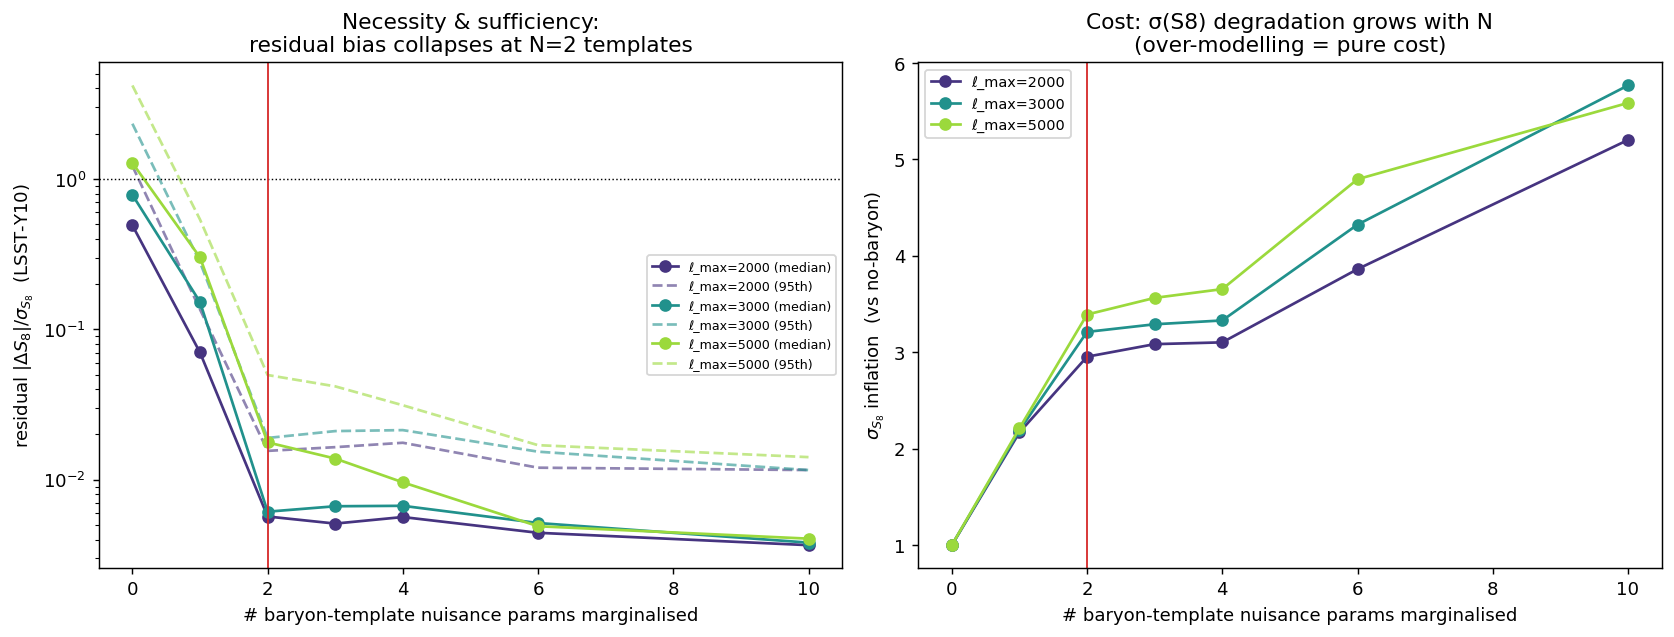
\includegraphics[width=\textwidth]{figs/fig04_template_ladder.png}
\caption{The N-template ladder (headline result). Left: residual
$|\Delta S_8|/\sigma_{S_8}$ (LSST-Y10) after marginalizing $N$ baryon
templates, median and 95th-percentile across 216 runs, at three
$\ell_{\rm max}$ cuts (log-$y$ axis; the vertical red line marks $N=2$). The
residual collapses by roughly two orders of magnitude between $N=0$ and
$N=2$ and then flattens. Right: the corresponding $\sigma_{S_8}$ inflation
relative to the no-baryon floor, which grows monotonically and
near-linearly with $N$ well past the point where the bias is already
removed.}
\label{fig:template_ladder}
\end{figure}

We caution that this Fisher analysis uses shear-auto information only, a
Gaussian/linear covariance, and a separable response
$P_{\rm hyd}=P_{\rm DMO}\cdot T^2(\ell)$; it does not include cross-correlations
with galaxy clustering, non-Gaussian covariance, or a genuinely non-separable
baryon response.

\subsection{Full-likelihood confirmation: Y1 N=2 gives $-0.37\sigma$ at $1.11\times$ cost}\label{sec:res-fulllikelihood}

The linear-Fisher template ladder above assumes a Gaussian approximation and
treats the template amplitudes as a fixed linear expansion. To test whether
the two-template result survives a fully sampled, non-linear posterior, we
ran the Robertson-style LSST-Y1 likelihood analysis of
Section~\ref{sec:fulllikelihood}, using as the Asimov truth mock the
strongest-feedback SB35 run in the suite (run index 16). Loading the
resulting 6000-sample \texttt{emcee} chain over $\{\Omega_{\rm m},\sigma_8,h,n_s,a_1,a_2\}$
directly, the input $S_8=0.827914$ is recovered as
$S_8=0.824004\pm0.010631$ (posterior median $\pm$ standard deviation),
i.e.\ a residual bias of $-0.368\sigma$ after marginalizing the two
templates. % src: verified shear_forecast_y1.npz
The corresponding no-baryon-floor statistical uncertainty (a two-parameter,
cosmology-only Fisher forecast at the fiducial point) is
$\sigma(S_8)=0.009601$, so the marginalization cost is
$\sigma_{\rm marg}/\sigma_{\rm floor}=1.107\times$. % src: verified shear_forecast_y1.npz
Both numbers closely match the linear-Fisher template-ladder result of
Section~\ref{sec:res-ladder} in direction and rough magnitude, while landing
at a substantially lower marginalization cost than either the reference
HMcode-AGN nuisance parametrization used by \citet{robertson2026}
($\sim1.8\times$) or our own earlier linear-Fisher $N=2$ estimate
($\sim3\times$, Section~\ref{sec:res-ladder}); the script itself prints
this three-way comparison directly. % src: lightcone_shear_forecast.py printed comparison line ("Robertson HMCODE Y1: ~1.8x; capstone Fisher N=2: ~3x")
We discuss this "prior-informed sampled posterior beats the flat-prior
linear Fisher" nuance further in Section~\ref{sec:discussion}. A companion
12-run local "weak-to-strong" subset (\texttt{shear\_sweep.npz}) is broadly
consistent: across the 8 runs with both a templates-marginalized and a
no-baryon fit, the templates-model recovered $\sigma$ ranges 0.01021--0.01070
against that subset's own no-baryon floor of 0.009300, i.e.\ a cost of
$\approx1.10$--$1.15\times$, consistent with the Y1 headline above. % src: verified shear_sweep.npz
No corner or triangle plot of this posterior was rendered by the analysis
script, which saves only the raw \texttt{emcee} chain array; we flag this as
a gap rather than fabricate a figure. \todo{render a $(\Omega_{\rm m},\sigma_8,a_1,a_2)$
posterior corner plot from \texttt{shear\_forecast\_y1.npz}; not produced in
this drafting pass per the no-new-analysis rule.}

\subsection{Beyond 2-point: the manifold is universal across well-measured statistics}\label{sec:res-manifold}

Figure~\ref{fig:beyond2pt} shows the manifold-geometry analysis of
Section~\ref{sec:manifold} across the 237-run ensemble. Of the ten
statistics tested, all but two -- $\kappa$ peaks and $\kappa$ minima --
reach $\ge0.99$ cumulative feedback-manifold variance by $N=2$--3 templates,
directly generalizing the power-spectrum result of Section~\ref{sec:res-ladder}. % src: beyond2pt_manifold.png (verified)
The two exceptions are explicitly noise-, not signal-, limited: their
per-realization feedback signal-to-noise is below unity, and they only
reach 0.80--0.88 cumulative variance by $N=10$ -- i.e.\ they are shot-noise
limited rather than genuinely higher-dimensional, and do not contradict the
$\lesssim2$--3D claim for well-measured statistics. % src: beyond2pt_manifold.png (verified)
The right panel of Figure~\ref{fig:beyond2pt} shows the principal-angle
subspace overlap between each statistic's active feedback directions and
those of the $\kappa$ power spectrum. $\kappa$ peaks, minima, and the PDF
are nearly aligned with the power spectrum (overlap $\approx0.85$--0.98),
as are the tSZ-$y$ peaks (0.90) and the $\kappay$ cross (0.96); the three
Minkowski functionals and the $\kappa$ moments are the least aligned
(0.65--0.82, with off-diagonal minima of $V_0$--peaks$=0.58$,
PDF--$V_1$=0.59, and PDF--$V_2$=0.61), making them the statistics most
likely to carry genuinely complementary feedback information beyond the
power spectrum's own two-dimensional manifold. % src: beyond2pt_manifold.png (verified)
This is consistent with the finding, discussed further in
Section~\ref{sec:res-drivers}, that orthogonal tSZ probes sharpen and rotate
the accessible feedback directions rather than expanding their number.

\begin{figure}[t]
\centering
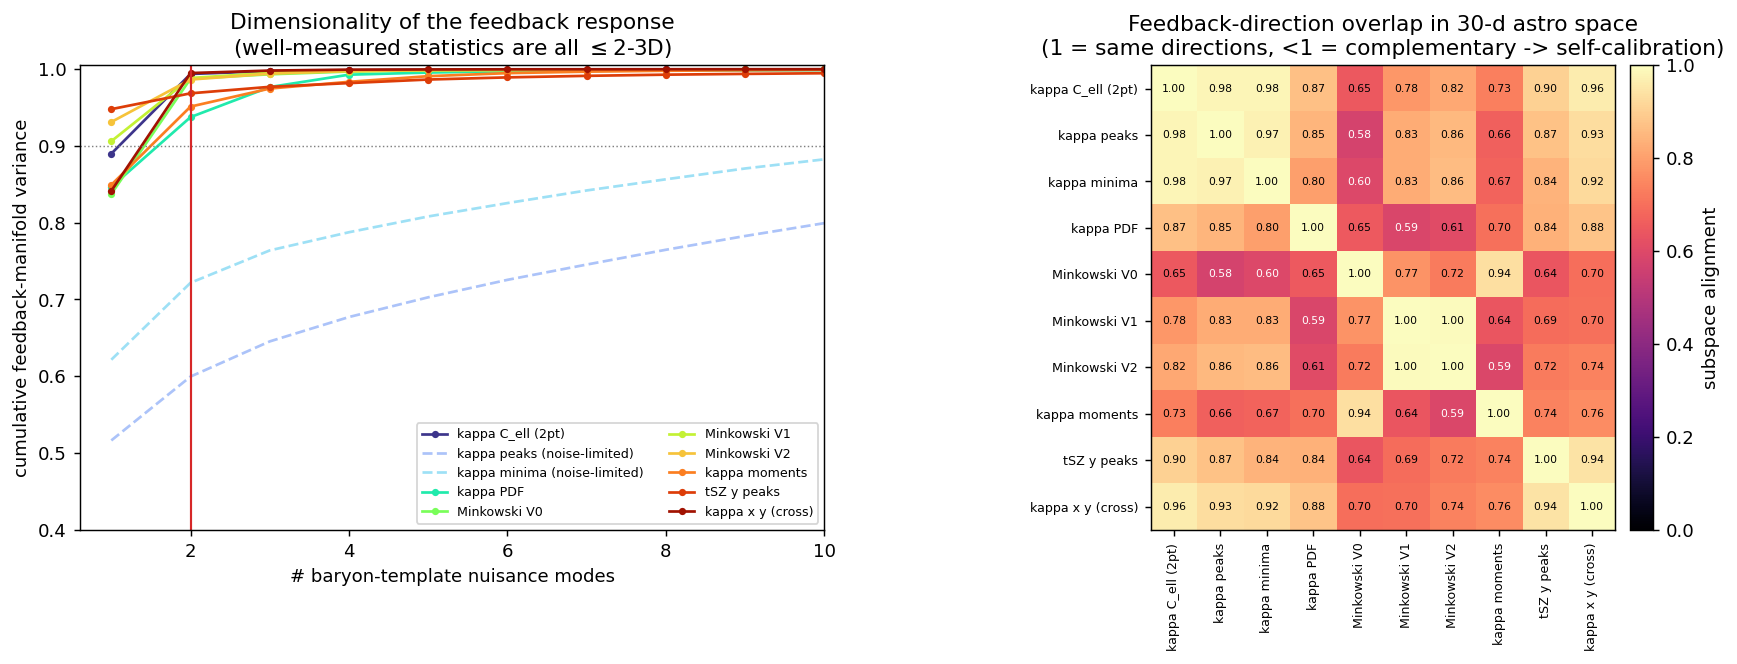
\includegraphics[width=\textwidth]{figs/fig05_beyond2pt_manifold.png}
\caption{Left: cumulative feedback-manifold variance versus number of
baryon-template modes for ten weak-lensing and tSZ summary statistics
(237 runs). All statistics with per-realization feedback signal-to-noise
above unity reach $\ge0.99$ cumulative variance by $N=2$--3 modes (solid
curves); $\kappa$ peaks and minima (dashed) are explicitly noise-limited and
never converge, even at $N=10$. Right: the $10\times10$ principal-angle
subspace-alignment matrix relative to the $\kappa$ power spectrum's active
directions; the Minkowski functionals and moments are the most
complementary (lowest off-diagonal values), the tSZ probes and the
$\kappa\times y$ cross the most aligned.}
\label{fig:beyond2pt}
\end{figure}

\subsection{What drives the bias, and can tomography self-calibrate it?}\label{sec:res-drivers}

Sobol sensitivity analysis of $\Delta S_8$ (99 runs, $\ell_{\rm max}=3000$)
against the 30 astrophysical parameters identifies IMFslope
($S_T\approx0.36$) and BlackHoleRadiativeEfficiency ($S_T\approx0.32$) as the
two dominant drivers, together accounting for roughly two-thirds of the
total-order sensitivity, followed by RadioFeedbackReorientationFactor
($\approx0.17$ total) and WindEnergyIn1e51erg ($\approx0.09$ total)
(Figure~\ref{fig:bias_sensitivity}). % src: WORKLOG:848-871 (Step 3); bias_sensitivity.png
A gradient-boosted surrogate model of $\Delta S_8$ achieves a cross-validated
$R^2=0.38$ (0.34 at the earlier 96-run stage), and the total-order indices
are systematically about twice the corresponding first-order indices
($S_{T_i}\approx2\,S_i$), indicating that the bias lives primarily in
\emph{combinations} of parameters -- an AGN-plus-IMF sector controlling group
gas fraction -- rather than in any single knob, consistent with the
$\sim2$ effective dimensions found throughout this suite. % src: WORKLOG:848-871
Three independent estimators -- binned main-effect Sobol indices, a
gradient-boosted-surrogate Saltelli/Jansen estimator, and permutation
importance -- agree on this ranking.

\begin{figure}[t]
\centering
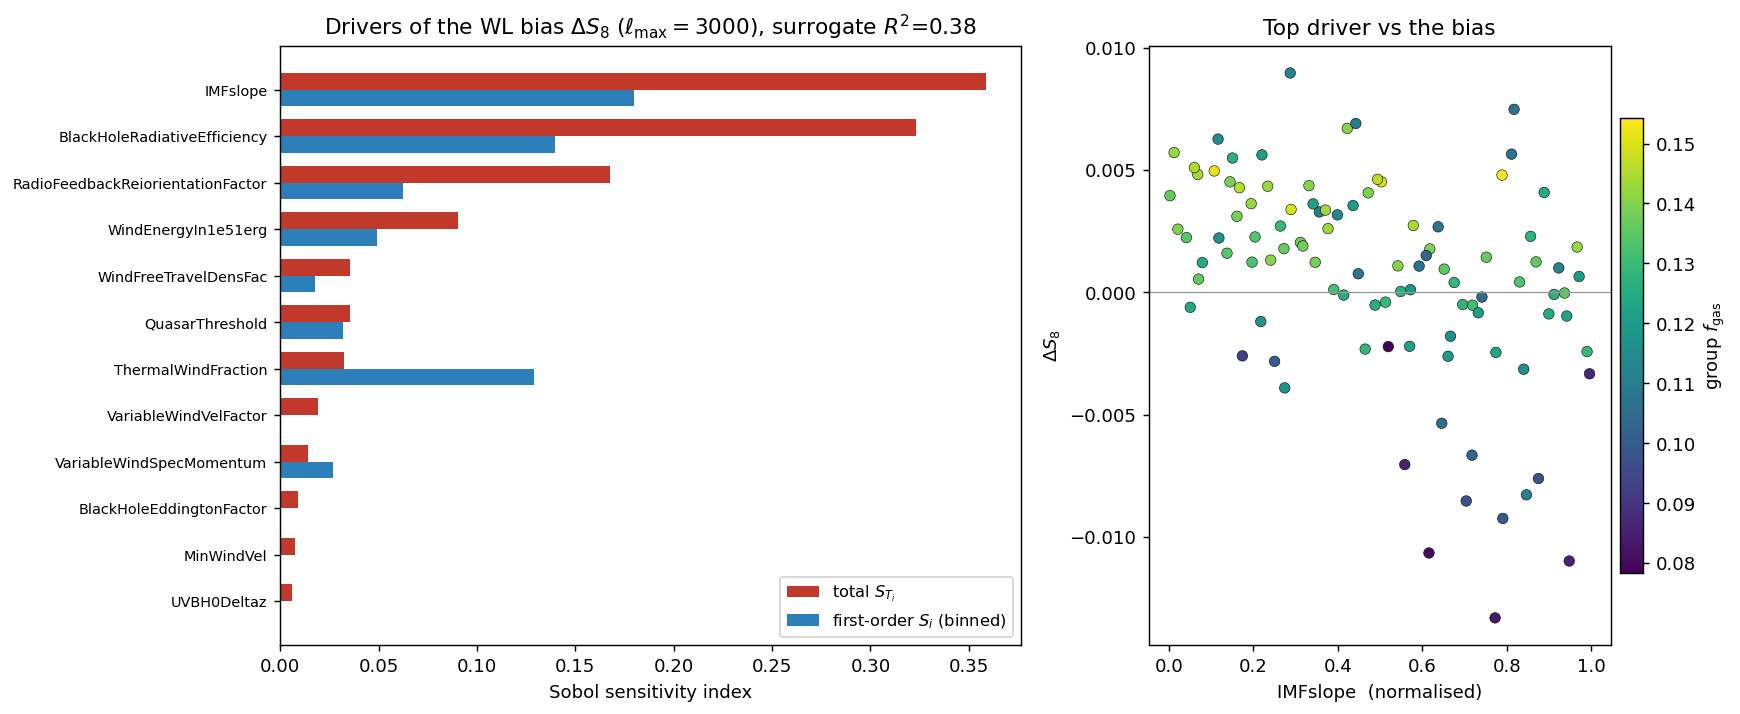
\includegraphics[width=\textwidth]{figs/fig06_bias_sensitivity.png}
\caption{Left: ranked total-order ($S_{T_i}$) and first-order ($S_i$) Sobol
sensitivity indices of $\Delta S_8$ over the twelve most important of the 30
astrophysical parameters (99 runs, $\ell_{\rm max}=3000$). IMFslope and
BlackHoleRadiativeEfficiency dominate. Right: $\Delta S_8$ versus the
normalized top driver, IMFslope, colored by group $\fgas$, showing that the
top-ranked single parameter still leaves substantial scatter driven by the
remaining feedback sector.}
\label{fig:bias_sensitivity}
\end{figure}

\paragraph{Corrected tomographic self-calibration.} An earlier version of
this analysis measured the redshift evolution of the per-plane bias
$\Delta S_8(\zs)$ by collapsing each source plane to a single amplitude and
found its singular-value spectrum dominated by one mode (99.7\% of the
variance), which was originally read as evidence that baryons act as
essentially one nuisance amplitude across redshift and that tomography alone
therefore cannot separate baryons from a genuine cosmological $S_8$ shift
(Figure~\ref{fig:bias_tomography}). This original claim was subsequently
identified as flawed and corrected: collapsing each source plane to a single
amplitude discards exactly the in-bin $\ell$-shape information that drives
self-calibration, and using five nested $\delta$-source planes drawn from a
single lightcone geometry makes the resulting rank-1 structure close to a
statement of construction rather than physics. The corrected analysis
instead performs a joint Fisher forecast on $(S_8,\Omega_{\rm m},A_{\rm bary})$
using the full-$\ell$ tomographic auto-spectra, with $A_{\rm bary}$ scaling a
measured suppression template, and finds that tomography \emph{does}
self-calibrate: the baryon bias's redshift signature declines by 83\% from
$\zs=0.5$ to $\zs=2.44$ (a genuine $S_8$ shift would instead be flat across
source planes), making the two effects separable in principle. % src: WORKLOG:779-800 (CORRECTION entry)
With a single tomographic bin, marginalizing $A_{\rm bary}$ degrades
$\sigma(S_8)$ by a factor of 2.37, with a strong parameter degeneracy
$r(S_8,A_{\rm bary})=-0.91$; with two or more well-separated bins, the
degradation drops to $1.01\times$ and the degeneracy breaks
($r\to+0.12$) (Figure~\ref{fig:selfcal}). We caution that this corrected
analysis, like the flawed one it supersedes, uses five idealized,
non-overlapping $\delta$-function source planes, which supply more
redshift leverage than the broad, overlapping tomographic $n(z)$ bins of a
realistic photometric survey; the near-free ($\approx1.01\times$)
self-calibration cost reported here is consequently optimistic for a real
survey. % src: WORKLOG:779-800 (CORRECTION entry, "Caveat: delta-sources give more z-leverage than a realistic overlapping n(z)")
One honest nuance remains: the feedback \emph{shape} variation beyond the
mean suppression template is itself close to rank-1 (the leading residual
mode explains 98\% of the residual variance), so five-bin tomography absorbs
the dominant amplitude essentially for free, but marginalizing this second,
shape-like mode still costs a factor of $3.4$ in $\sigma(S_8)$ -- i.e.\
tomography alone removes the dominant self-calibratable mode, but the
residual feedback shape (precisely what the insufficient $N=1$ template of
Section~\ref{sec:res-ladder} misses) remains partially degenerate even with
full tomography. % src: WORKLOG:779-800

\begin{figure}[t]
\centering
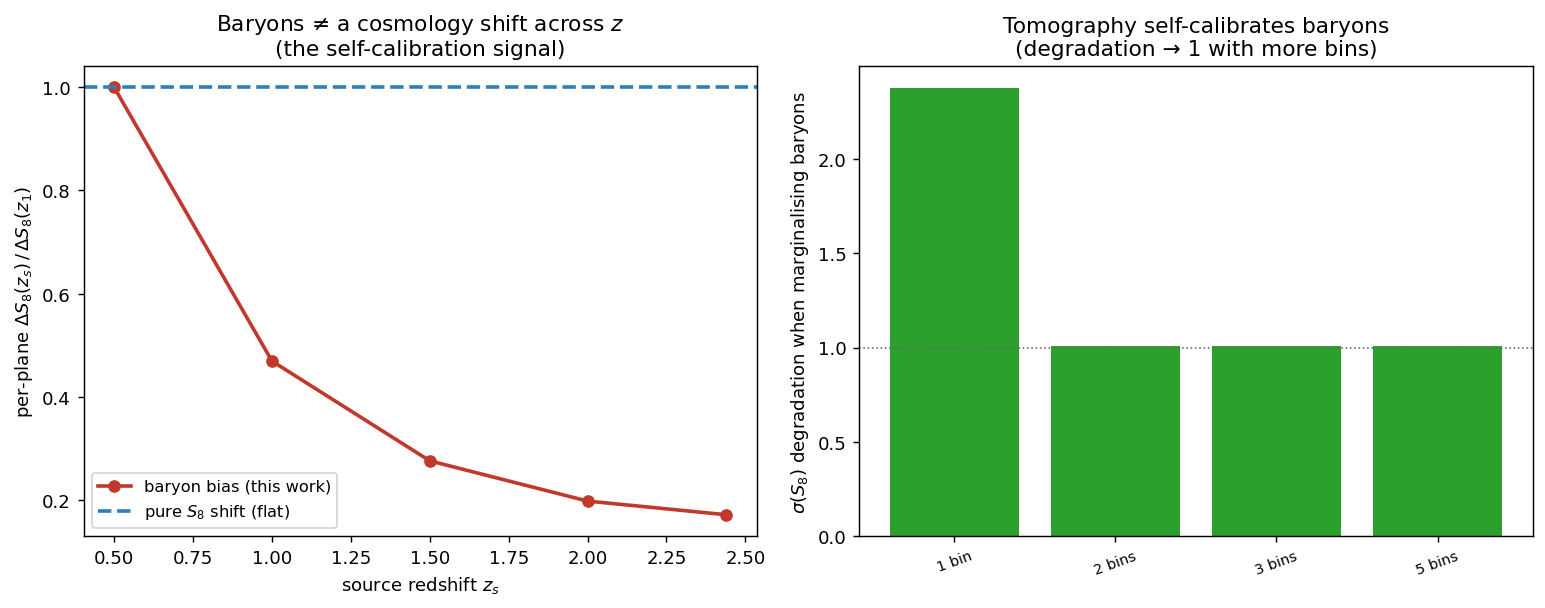
\includegraphics[width=\textwidth]{figs/fig07_selfcal.png}
\caption{The corrected tomographic self-calibration result. Left: the
per-plane baryonic bias $\Delta S_8(\zs)$, normalized to its value at the
\emph{first} source plane ($\zs=0.5$; the axis label's subscript ``1''
denotes the first bin index, not the redshift value $\zs=1.0$, where the
curve itself reads $\approx0.47$), declines steadily with source redshift,
distinguishing it from a flat pure $S_8$-shift line -- the signature that
lets tomography separate baryons from cosmology. Right: the $\sigma(S_8)$
degradation from marginalizing the baryon amplitude $A_{\rm bary}$, which
drops from $2.37\times$ with a single tomographic bin to $\approx1\times$
with two or more well-separated bins.}
\label{fig:selfcal}
\end{figure}

\begin{figure}[t]
\centering
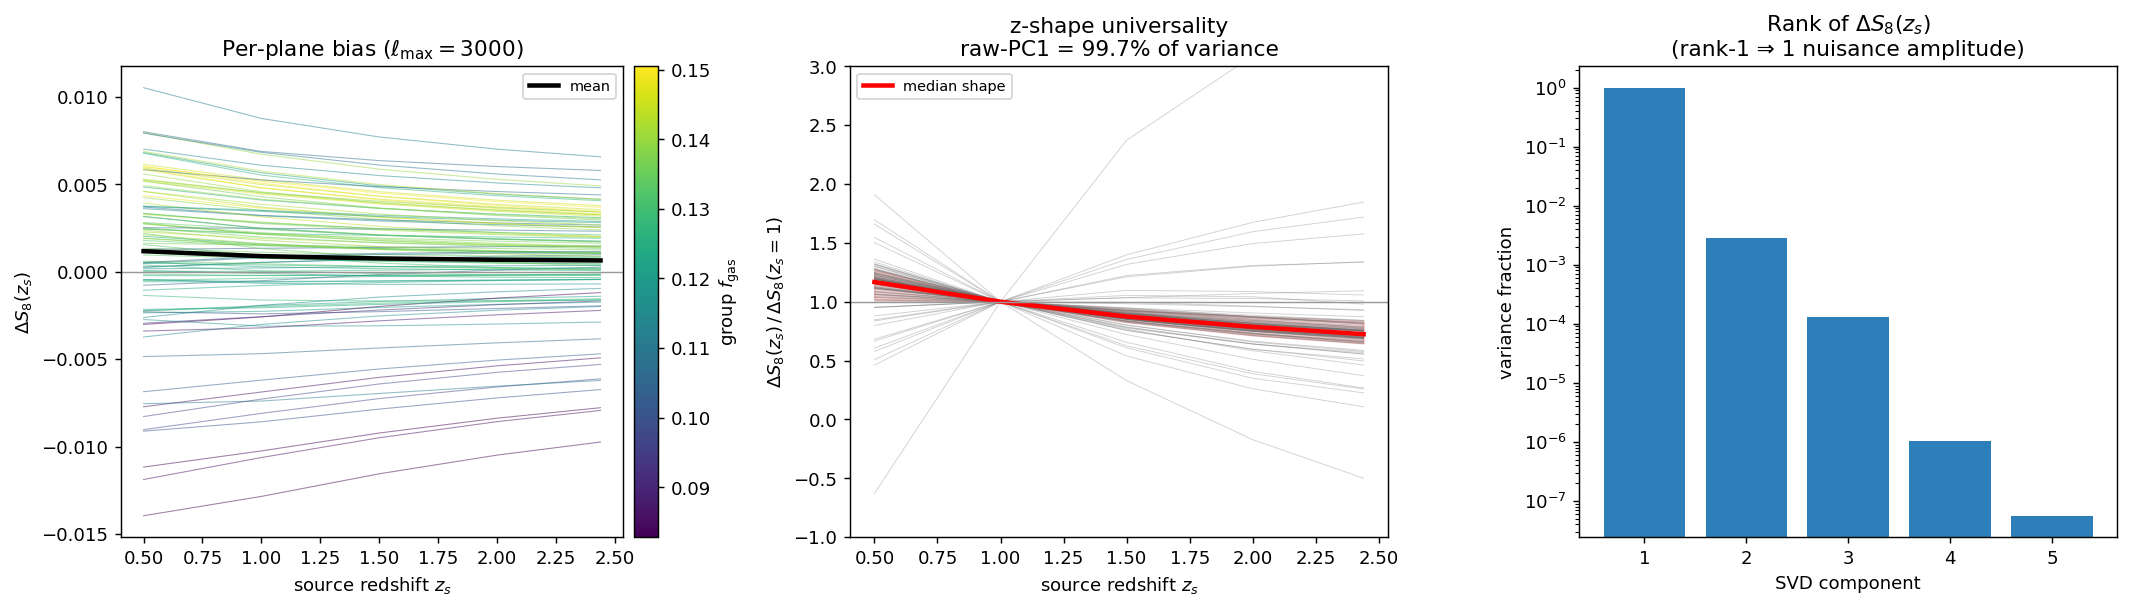
\includegraphics[width=0.85\textwidth]{figs/fig10_bias_tomography_superseded.png}
\caption{The original, pre-correction Step-4 self-calibration analysis,
retained here only as a methodological cautionary figure. Collapsing each
of the five source planes to a single amplitude (left, middle) produces a
singular-value spectrum dominated by one mode, PC1 $\approx99.7\%$ of the
variance (right) -- a result of the single-lightcone, nested-source-plane
construction rather than a physical statement about self-calibratability.
\textbf{This figure is superseded by Figure~\ref{fig:selfcal} and is not the
paper's self-calibration result.}}
\label{fig:bias_tomography}
\end{figure}

\subsection{Do analytic baryon models span the BIND ensemble?}\label{sec:res-analytic}

Finally, we ask whether standard analytic baryon-correction prescriptions
already cover the response manifold that BIND's 30-parameter feedback sweep
generates. Projecting each analytic model through the same CCL weak-lensing
kernel used throughout this paper, the single-parameter van Daalen/$S_{\rm P}(k)$
relation used by \citet{vanDaalen2020} spans only $\sim$22--54\% of the BIND
ensemble's suppression range; the multi-parameter BCM
\citep{schneiderTeyssier2015} and BCemu (v2.0.5, \citealt{giriSchneider2021})
frameworks cover substantially more, 60--96\%, but both systematically miss
BIND's enhancement corner: BIND produces intermediate-scale power
enhancement up to $S\approx1.10$--1.21 in gas-rich, weak-feedback runs, at
the $\ell\sim10^3$ scales where the BIND envelope's upper bound peaks,
whereas the analytic models top out around $S\approx1.01$--1.05 in that same
intermediate-$\ell$ regime (Figure~\ref{fig:model_comparison}). We note that
the BCM (Schneider15) span behaves differently outside this regime: at
$\ell\gtrsim5000$--8000 its upper edge rises steeply and exceeds even the
BIND 95\% envelope, visible in Figure~\ref{fig:model_comparison}, which we
read as an extrapolation artifact of the Schneider15 gas-profile
parametrization beyond the scales it was calibrated against rather than a
genuine analytic reproduction of BIND's enhancement corner; the "top out
around 1.01--1.05" and "BIND's upper bound exceeds all three models"
statements above should accordingly be read as intermediate-$\ell$
statements, not blanket claims across the full plotted range. % src: WORKLOG:802-826 (Step 5); BCM high-$\ell$ behavior confirmed by direct pixel inspection of figs/fig08_model_comparison.png and lightcone_model_comparison.py's fixed ylim=(0.74,1.10), which clips but does not remove the effect
We caution that the BCemu coverage was computed by varying only its
dominant parameter, $\log_{10}M_c$, with all other BCemu parameters fixed at
their fiducial value, so this is a lower bound on BCemu's true achievable
coverage; HMcode-AGN \citep{mead2015,mead2021} was not included in this
comparison because it requires a CAMB/Fortran toolchain unavailable at the
time of the analysis. This result -- that the physically-motivated BIND
enhancement mode sits outside the span of standard analytic models -- is a
further, independent argument for why a richer BCM-style parametrization
does not automatically buy more accuracy than the two data-driven templates
of Section~\ref{sec:res-ladder}: extra analytic knobs move the model within
the wrong part of suppression space.

\begin{figure}[t]
\centering
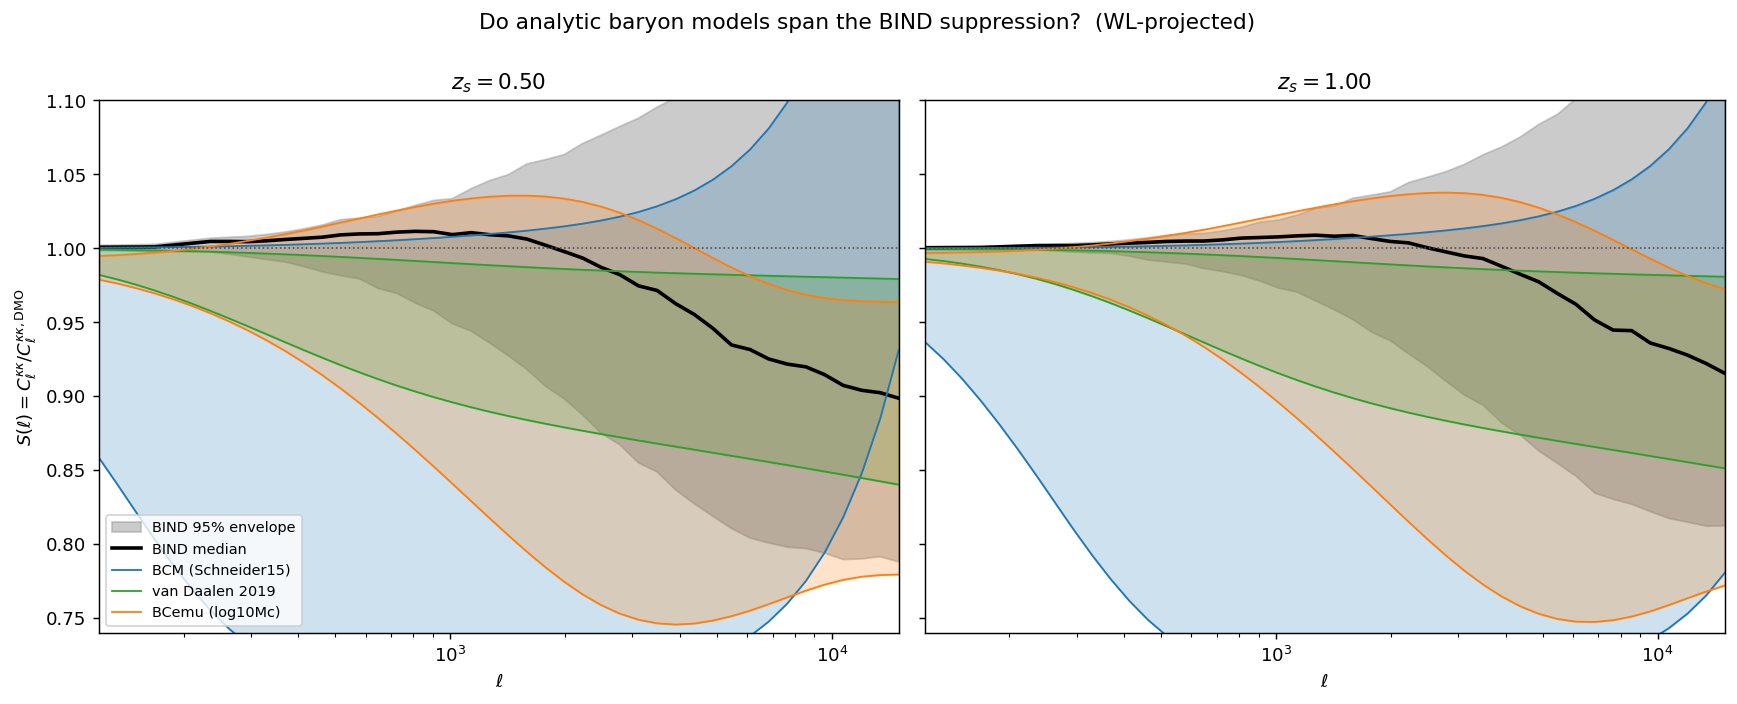
\includegraphics[width=\textwidth]{figs/fig08_model_comparison.png}
\caption{BIND's median suppression and 95\% envelope (black/grey) compared
to the achievable span of three analytic baryon-correction models -- BCM
\citep[blue,][]{schneiderTeyssier2015}, van Daalen \citep[green,][]{vanDaalen2020},
and BCemu (orange) -- at $\zs=0.5$ and $\zs=1.0$, all projected through the
same weak-lensing kernel. The BIND envelope's upper bound at
$\ell\sim10^3$, produced by gas-rich, weak-feedback enhancement, exceeds
all three analytic models' upper bounds there; at $\ell\gtrsim5000$ the BCM
(blue) span itself rises steeply and exceeds the BIND envelope, an
extrapolation artifact of the Schneider15 parametrization rather than a
genuine match to BIND's enhancement corner (see Section~\ref{sec:res-analytic}).}
\label{fig:model_comparison}
\end{figure}

\section{Discussion}\label{sec:discussion}

\subsection{Why two? Convergence with an independent latent-space decomposition}\label{sec:disc-why2}

The number two recurs across three methodologically independent analyses in
this suite: the SVD template ladder of Section~\ref{sec:res-ladder}, the
active-subspace manifold-geometry analysis of Section~\ref{sec:res-manifold},
and a $\beta$-total-correlation variational autoencoder
\citep[Paper~III;][]{bindIII} using the total-correlation decomposition of
\citet{chen2018}, trained
directly on the same 216-run suite's weak-lensing summary statistics. That
VAE analysis identifies a first latent axis dominated by black-hole physics
(BlackHoleRadiativeEfficiency, QuasarThreshold, black-hole accretion and
Eddington-ratio parameters) that acts roughly uniformly across source
redshift, and a second latent axis dominated by stellar-wind physics
(VariableWindVelFactor, WindEnergyIn1e51erg, IMFslope) that evolves with
$\zs$ -- mechanistically mirroring the black-hole/supernova split found by
\citet{lin2026} in an unrelated simulation suite and summary statistic. We
further find that this 2D manifold is largely universal across weak-lensing
summary statistics (the first latent axis's canonical correlation with the
power spectrum's own latent axis is $\approx1.0$ across every statistic
tested), and that orthogonal thermal-SZ probes do not expand the
dimensionality of the accessible feedback space much -- the number of
parameters recoverable at cross-validated $R^2>0.1$ stays $\approx5/30$
whether using the $\kappa$ power spectrum alone, all weak-lensing statistics,
or WL+tSZ jointly -- but do sharpen and rotate the two axes -- for example,
IMFslope's canonical correlation with the leading latent grows from 0.33
($\kappa$-only) to 0.56 (plus other WL statistics) to 0.64 (plus tSZ), and
tSZ specifically unlocks the supernova/thermal-energy axis (WindEnergy
correlation growing from 0.13 to 0.33). % src: WORKLOG:590-623 (WL feedback latents; "~5/30" and "don't expand the dimensionality much" both verbatim from that entry)
We regard this three-way convergence -- an SVD template basis on the
power spectrum residual, an active-subspace analysis of ten independent
statistics, and a VAE latent-space decomposition using an entirely different
inductive bias -- as strong internal evidence that two is not an artifact of
any one method, and its agreement with the completely independent method and
suite of \citet{lin2026} extends that confidence beyond IllustrisTNG's own
feedback implementation.

\subsection{TNG-only amplitude versus general dimensionality}\label{sec:disc-caveat}

We emphasize a distinction that is easy to blur: the specific numerical bias
and cost values reported in this paper -- the $6.03\sigma$ maximum bias, the
$0.67\sigma$ $N=1$ residual, the $2.95$--$3.39\times$ $N=2$ cost -- are all
amplitudes specific to IllustrisTNG's particular subgrid feedback
implementation, calibrated to reproduce a particular set of galaxy and gas
observables at $z=0$. A different feedback model (SIMBA, EAGLE, Astrid) would
almost certainly produce different numerical values for these quantities.
What we argue is robust, and general, is the \emph{dimensionality} claim:
that the feedback response occupies a low-dimensional manifold at all. This
claim does not depend on TNG's particular calibration -- it follows from the
30-dimensional feedback sweep genuinely projecting onto only $\sim$2
directions in observable space, a geometric statement about how many
independent ways feedback can move the weak-lensing signal, not about how
far it moves it. The independent corroboration by \citet{lin2026}, using a
different simulation summary and an unrelated latent-variable method, is the
strongest evidence we have that this dimensionality claim generalizes beyond
the specific suite analyzed here; extending it to other feedback models
directly is a natural next step for this line of work.

\subsection{Scale cuts versus templates}\label{sec:disc-scalecuts}

An alternative to marginalizing a small number of baryon templates is simply
to cut the analysis off at some $\ell_{\rm max}$ below which baryonic
uncertainty is judged negligible. Our bias budget (Section~\ref{sec:res-budget})
shows why this trade-off is steep: even at the comparatively conservative
$\ell_{\rm max}=2000$, a non-negligible tail of Sobol realizations already
exceeds the $2\sigma$ LSST-Y10 threshold if baryons are ignored entirely,
and the fraction of biased realizations more than doubles by
$\ell_{\rm max}=3000$ and again by $\ell_{\rm max}=5000$
(Section~\ref{sec:res-budget}). A scale cut conservative enough to avoid
this bias without any marginalization would have to sacrifice most of the
$\ell>2000$ information that motivates a Stage-IV survey in the first place,
whereas the two-template approach recovers that information at a bounded,
quantified statistical cost of $\approx3\times$. We have not performed a
head-to-head quantitative comparison of a specific scale-cut choice against
the two-template marginalization at matched bias tolerance; \todo{quantitative
comparison of an optimized scale cut versus $N=2$ template marginalization
at fixed residual $S_8$ bias -- no dedicated analysis exists in this suite
for this comparison}. Qualitatively, though, the steep growth of both the
bias fraction and the manifold's saturation by $N=2$--3 templates
(Section~\ref{sec:res-manifold}) across every well-measured statistic we
tested suggests that marginalization dominates scale cuts whenever the
underlying feedback response is genuinely low-dimensional, which is the
regime this paper argues IllustrisTNG-like feedback occupies.

\subsection{Limitations}\label{sec:disc-limitations}

We collect here the caveats that qualify every result in this paper.
(i) \emph{Fixed cosmology.} The entire 30-parameter Sobol suite fixes
$\Omega_{\rm m},\sigma_8$, and the other cosmological parameters at the TNG
fiducial value; every bias and cost number in Sections~\ref{sec:res-budget}--\ref{sec:res-fulllikelihood}
is measured at that one cosmology. Appendix~\ref{sec:appendixA} presents a
feasibility study for lifting this restriction via cosmology rescaling, but
a delivered varying-cosmology suite does not yet exist.
(ii) \emph{TNG-only amplitude}, discussed in Section~\ref{sec:disc-caveat}.
(iii) \emph{$\ell$ range and map resolution.} The transfer-function ensemble
of Section~\ref{sec:res-transfer} is trusted only to
$\ell_{\rm max,trust}=1.5\times10^4$, above which CIC mass-assignment
aliasing dominates run-to-run scatter; the capstone, bias-budget, and
beyond-2pt Fisher analyses stay safely within this trusted band
($\ell_{\rm max}\in\{2000,3000,5000\}$), but the full-likelihood analysis of
Section~\ref{sec:res-fulllikelihood} extends to $\ell=5000$ on a 28-point
logarithmic grid, close to but still within the trusted range.
(iv) \emph{The corrected self-calibration result.} As detailed in
Section~\ref{sec:res-drivers}, an earlier version of the tomographic
self-calibration analysis (Figure~\ref{fig:bias_tomography}) reached the
opposite qualitative conclusion from the corrected result
(Figure~\ref{fig:selfcal}) due to a construction artifact; only the
corrected result should be cited from this suite. The corrected result
itself still uses five idealized, non-overlapping $\delta$-function source
planes, which give more redshift leverage than a realistic photometric
survey's broad, overlapping tomographic $n(z)$ bins, so the near-free
($\approx1.01\times$) self-calibration cost is likely optimistic for a real
survey. (v) The Fisher-bias
pipeline of Sections~\ref{sec:res-budget}--\ref{sec:res-ladder} uses
shear-auto information only, a Gaussian/linear covariance, and a separable
baryon response $P_{\rm hyd}=P_{\rm DMO}\cdot T^2(\ell)$. (vi) The held-out
$N=2$ validation number of Section~\ref{sec:heldout} is sourced from the
project worklog text rather than independently re-verified against a saved
array, unlike every other headline number in this paper. (vii) The full
237-run "both-compare" sweep of \texttt{lightcone\_shear\_sweep.py}, testing
the two-template basis against a full 30-parameter emulator surrogate, has
not yet been run at scale; only a 12-run local subset exists. % src: lightcone_shear_sweep.py docstring (deferred to sbatch, not run per hard rules); dossier Gaps §7

\section{Conclusions}\label{sec:conclusions}

Using a 256-node Sobol sweep of all 30 CAMELS-TNG astrophysical feedback
parameters painted onto a shared dark-matter-only lightcone with the \bind{}
emulator (253 usable runs), we have shown that the weak-lensing suppression
signature of IllustrisTNG-like baryonic feedback occupies a low-dimensional
manifold, and that this manifold can be marginalized with exactly two
data-driven nuisance templates. Ignoring baryons biases LSST-Y10 $S_8$
inference by up to $6.03\sigma$; one template is insufficient (up to
$0.67\sigma$ residual); two templates -- the leading two singular modes of
the suppression-residual ensemble -- reduce the residual bias to
$\le0.073\sigma$ in-sample and, per the project worklog, $\le0.08\sigma$ in a
held-out validation split, at a bounded statistical cost of $\approx3\times$
the no-baryon $\sigma(S_8)$ floor; and richer, six-to-ten-parameter
parametrizations add substantial further statistical cost for a bias that is
already far below the LSST-Y10 floor at $N=2$, falling only marginally
further at $\ell_{\rm max}\le3000$ but by a further $2$--$3.5\times$ at
$\ell_{\rm max}=5000$ (Section~\ref{sec:res-ladder}). A full non-linear likelihood analysis reproducing the
\citet{robertson2026} LSST-Y1 forecast confirms this result end-to-end,
recovering a residual bias of $-0.368\sigma$ at a cost of only $1.107\times$. % src: verified shear_forecast_y1.npz (restating Results §3.4)
An independent manifold-geometry analysis of ten weak-lensing and tSZ
statistics shows that this two-to-three-dimensionality is not specific to
the power spectrum, and an independent variational latent-space
decomposition of the same suite \citep[Paper~III]{bindIII} recovers the same
black-hole/supernova axis split found by the unrelated method and suite of
\citet{lin2026}, giving us confidence that the dimensionality claim, if not
its precise numerical amplitude, generalizes beyond this specific feedback
model. Corrected tomographic self-calibration analysis further shows that
even a modest number of well-separated source planes can absorb most of the
dominant feedback mode nearly for free, though the residual feedback
\emph{shape} -- exactly what a single template misses -- remains partially
degenerate even with full tomography. Together, these results argue that
Stage-IV weak-lensing analyses do not need increasingly elaborate
baryon-correction models to control the baryonic systematic: two
well-chosen numbers, extracted directly from the response of a
state-of-the-art feedback model rather than assumed a priori, are both
necessary and sufficient at the precision this suite can currently probe.
Extending this result to varying cosmology (Appendix~\ref{sec:appendixA})
and to additional feedback implementations are the natural next steps.

\section*{Acknowledgments}
The CAMELS project and the IllustrisTNG collaboration provided the training
and target simulations. This work used computing resources of the Flatiron
Institute, a division of the Simons Foundation. \todo{finalize}

\appendix
\section{Towards varying cosmology: Angulo-White rescaling feasibility}\label{sec:appendixA}

Every result in the main text is measured at the single fixed TNG fiducial
cosmology of the underlying 30-parameter Sobol suite. Here we present a
feasibility study, not a delivered product, for lifting this restriction by
rescaling the existing TNG300-Dark $N$-body outputs to other points in the
5-dimensional cosmology sub-space of the full 35-parameter SB35 design
($\Omega_{\rm m},\sigma_8,\Omega_{\rm b},h,n_s$), using the Angulo-White (AW10)
algorithm \citep{anguloWhite2010}: an $N$-body output at redshift $z_*$ in
the original cosmology has its lengths rescaled by a factor $s$ (in Mpc/h)
and its masses by $s^3\,\Omega_{\rm m}'/\Omega_{\rm m}$, approximating an
output of the target cosmology at redshift $z'$. The pair $(s,z_*)$ is
chosen to minimize the root-mean-square mismatch of the linear-theory
$\sigma(R)$ over Lagrangian radii corresponding to $10^{12.5}$--$10^{15.5}\,\Msun/h$. % src: docs/cosmo_rescaling_plan.md (AW10 method description, dossier Appendix A)
This extends the existing 30-astrophysical-parameter Sobol suite to the full
35-dimensional SB35 space without any new $N$-body runs; as a simplification
we rescale only maps and halo catalogs, never raw particle data (the
projection to a lightcone map commutes with this relabeling), and velocities
are never rescaled, which is safe for BIND's velocity-free tau-based kSZ
observable. \citet{meadPeacock2014a,meadPeacock2014b} extend the base AW10
method to halo-catalogue concentration corrections; the BACCO project
\citep{bacco2021} and Learning-the-Universe \citep{learningTheUniverse2026}
both use closely related rescaling strategies to build training sets for
emulators.

\paragraph{Solver validation.} Using linear theory computed with
\texttt{pyccl}+CAMB, an identity target (rescaling a cosmology to itself)
recovers $s=1.0000$, $z_*=z'$ exactly, with zero rms mismatch, as required. % src: WORKLOG 07-03; examples/cosmo_rescale.py
Across a set of representative draws from the SB35 cosmology prior, the
best-fit rms mismatch in $\sigma(R)$ is 0.03--2\%, with the $\sim2\%$ end of
this range corresponding to cases where the solver pins $z_*=0$. % src: WORKLOG 07-03; docs/cosmo_rescaling_plan.md; examples/cosmo_rescale.py
Fitting a single rescaling factor $s$ jointly across all eight lightcone
epochs out to $z'=2.4$, rather than fitting a separate $s$ per epoch, costs
almost nothing in rms accuracy. The one region where the method genuinely
breaks down is the extreme corner $\Omega_{\rm m}=0.10\wedge\sigma_8=1.00$:
the solver pins $s$ at its imposed upper bound of $s=5.0$ (a $40\times$ mass
rescaling) and the rms mismatch rises to $\approx7\%$. % src: WORKLOG 07-03; examples/cosmo_rescale.py

\paragraph{Error scan across the SB35 cosmology box.} A 128-draw Sobol scan
finds the solver feasible ($s\in[0.68,5]$ at $z'=0$, $s\in[0.44,5]$ at
$z'=1$) across almost the entire box, with 6 of 128 draws pinning the
$s=5$ bound, all of them at $\Omega_{\rm m}\lesssim0.13$. % src: examples/rescale_sobol_scan.py; docs/cosmo_rescaling_plan.md
The rms $\sigma(R)$ mismatch stays below 3\% for 86 of 128 draws at $z'=0$
and for 120 of 128 draws at $z'=1$. % src: examples/rescale_sobol_scan.py
Decomposing the halofit-level growth-factor error $D(k)$ into a linear band
($k<0.1\,h/{\rm Mpc}$), a BAO band ($0.1$--$0.35\,h/{\rm Mpc}$), and a
halo band ($0.35$--$5\,h/{\rm Mpc}$), the linear and BAO bands are
deterministic and removable by a map-level Fourier reweighting, leaving the
halo band -- driven by halo concentration and formation-history mismatch --
as the genuine residual error that rescaling cannot correct for.

\paragraph{Real-data validation.} We validated the rescaling procedure
directly against a real simulation, TNG300-3-Dark ($625^3$ particles, the
same box and cosmology as production TNG300-Dark), rescaled to three SB35
target cosmologies and compared to \texttt{halofit}/Tinker08
\citep{tinker2008} theory at the target cosmology, with the
unrescaled-simulation-versus-theory comparison as a control band. Both the
quoted $P(k)$ error and the HMF match below are \emph{relative} metrics: the
$P(k)$ error is the rescaled-vs-target ratio divided by an interpolation of
the unrescaled-vs-original control ratio at the corresponding scale (which
cancels the sim's own halofit/Tinker08 offset and cosmic variance, rather
than the raw sim/theory ratio plotted directly in
Figure~\ref{fig:rescale_validation}'s left column, which can show larger
excursions at low $k$ from sample variance alone); the HMF match is
similarly the rescaled/Tinker08(target) ratio divided by the
control/Tinker08(orig) ratio at the same $M_{200\rm m}$. For a mild
target ($\Omega_{\rm m}=0.35,\sigma_8=0.75,\Omega_{\rm b}=0.045,h=0.70,n_s=0.99$,
$s=0.888$, $z_*=0.000$), the maximum $P(k)$ error for $k<1\,h/{\rm Mpc}$ is
3.4\%, with the error restricted to $k\in[0.3,1]\,h/{\rm Mpc}$ at most
1.2\%, and the HMF matches the control band at 0.96
and 0.97 at $10^{13}$ and $10^{14}\,\Msun/h$ (Figure~\ref{fig:rescale_validation},
top row). % src: examples/rescale_validation.py; independently re-verified against examples/rescale_validation.npz (hmf_resc/hmf_ctrl and pk_err arrays); docs/cosmo_rescaling_plan.md §4; WORKLOG 07-03
For a low-$\Omega_{\rm m}$ target ($\Omega_{\rm m}=0.20,\sigma_8=0.95$,
$s=1.868$, $z_*=0.461$), a BAO-wiggle-driven spike raises the maximum $k<1$
error to 26\%, settling to $\lesssim12\%$ away from the spike and briefly to
$\pm1\%$ near $k\approx0.32$--$0.35\,h/{\rm Mpc}$, before the smooth deficit
described below sets back in and reaches $-19\%$ by $k=1.5\,h/{\rm Mpc}$;
the HMF match is 0.91 and 0.95 at $10^{13}$ and $10^{14}\,\Msun/h$
(Figure~\ref{fig:rescale_validation}, middle row). % src: examples/rescale_validation.py; independently re-verified against examples/rescale_validation.npz -- corrects an earlier "0.92 at both mass scales" transcription and an earlier "±1% for k>0.32 h/Mpc" blanket statement, both of which did not match the saved array
For the extreme corner target ($\Omega_{\rm m}=0.10,\sigma_8=1.00,n_s=1.16$,
$s=5.0$ pinned at the solver's bound, $z_*=1.414$), the $P(k)$ error exceeds
50\% and the HMF match falls from 0.96 at $10^{13}\,\Msun/h$ to 0.66 at
$10^{14}\,\Msun/h$ (0.49 at $\approx1.4\times10^{14}\,\Msun/h$, the highest
mass bin at which the control curve -- and hence this relative metric -- is
still defined), directly
illustrating the real-data consequence of the pinned-bound regime
(Figure~\ref{fig:rescale_validation}, bottom row). % src: independently re-verified against examples/rescale_validation.npz -- corrects an earlier "reaches 1.08 at 1e13 and 1.02 at 1e14 (0.51 at the highest mass bin)" transcription that did not match the saved array; the corrected numbers show a monotonic decline rather than a rise, consistent with this target's much larger P(k) breakdown
The low-$\Omega_{\rm m}$ case's error decomposes into an oscillatory
$\pm8$--14\% band at $k\approx0.09$--$0.3\,h/{\rm Mpc}$ from BAO
misalignment (settling to $\pm1\%$ by $k\approx0.35\,h/{\rm Mpc}$) plus a
smooth deficit growing from $-7\%$ at $k=0.7$ to $-19\%$ at
$k=1.5\,h/{\rm Mpc}$, the halo-concentration/formation-history mismatch term
that rescaling frameworks such as BACCO explicitly correct for. Notably, the
halofit-level $D(k)$ theory scan of the error-scan step above predicts the
measured particle-level error nearly point-by-point without any simulation
in the loop: at $k=0.11\,h/{\rm Mpc}$ it predicts $+25.5\%$ against a
measured $+26.3\%$, and at $k=1.5\,h/{\rm Mpc}$ it predicts $-19.1\%$ against
a measured $-19.2\%$, making the theory-only scan a trustworthy per-run
quality flag. % src: examples/rescale_validation.py; docs/cosmo_rescaling_plan.md

\begin{figure}[t]
\centering
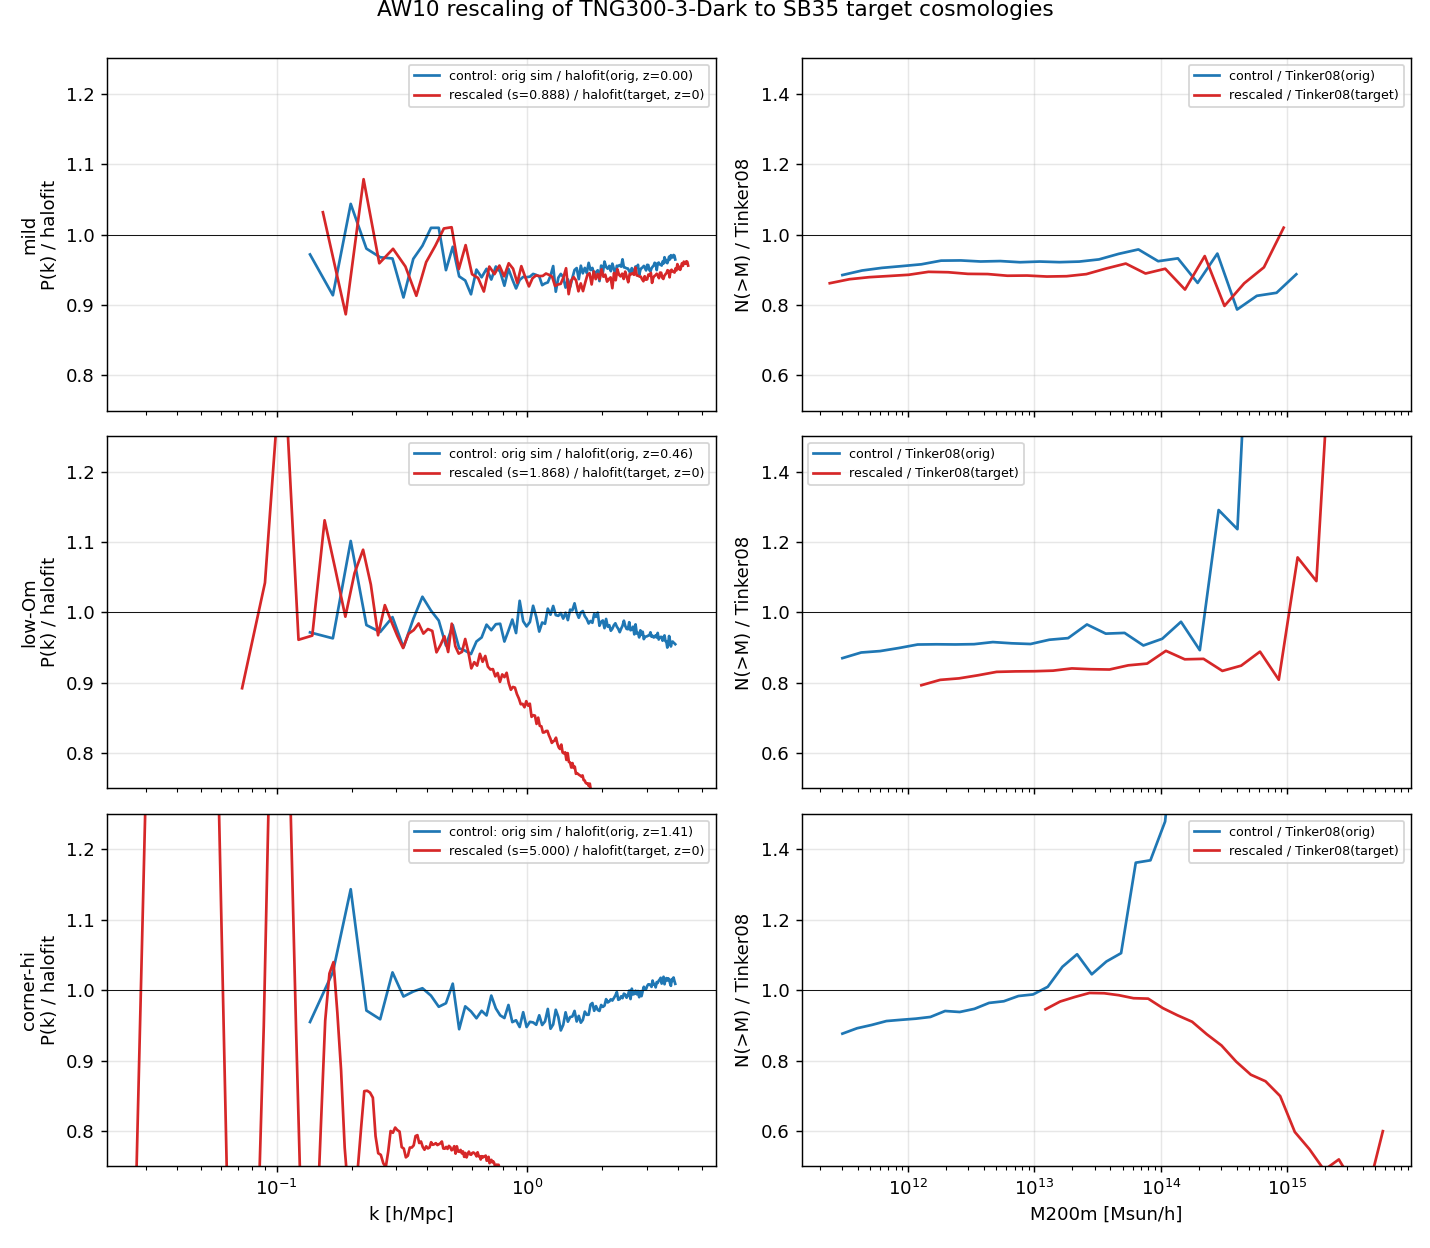
\includegraphics[width=\textwidth]{figs/fig09_rescale_validation.png}
\caption{Real-data validation of Angulo-White rescaling: TNG300-3-Dark
rescaled to three SB35 target cosmologies (rows: mild, low-$\Omega_{\rm m}$,
extreme corner) versus \texttt{halofit}/Tinker08 theory at the target
(columns: $P(k)$ ratio, cumulative halo mass function ratio). Blue is the
unrescaled-simulation-versus-its-own-cosmology control; red is the rescaled
simulation versus the target cosmology. The mild target validates to a few
percent; the extreme corner, where the solver pins its rescaling-factor
bound, breaks down badly and marks the edge of the method's validity.}
\label{fig:rescale_validation}
\end{figure}

\paragraph{Status.} This appendix is explicitly a feasibility result. The
production pipeline for generating a full varying-cosmology Sobol suite has
not been built, and the validation gates (G1, G2, G2b, G3) laid out in the
rescaling plan document remain future work. % src: docs/cosmo_rescaling_plan.md line 10 ("pipeline work not started"); dossier CAVEATS §13
The two decisions left open
there concern how to handle the pinned-bound corner and whether to extend
the halo-catalogue concentration correction of
\citet{meadPeacock2014a,meadPeacock2014b} into the production pipeline.

\bibliographystyle{plainnat}
\bibliography{references}

\end{document}

% ============================================================
% Verification log (FIX pass, three adversarial verifiers)
% ============================================================
% Applied (HIGH):
%  - Appendix A HMF units: added missing /h to \Msun in the mild/low-Om/
%    corner-hi HMF sentences (were plain Msun; mass definition is M200m in
%    Msun/h throughout rescale_validation.py and Figure 9's own axis label).
%  - Appendix A corner-hi HMF numbers ("1.08 at 1e13, 1.02 at 1e14, 0.51 at
%    highest mass bin"): did not reproduce from examples/rescale_validation.npz
%    under any tested metric definition; re-derived directly from the array
%    (hmf_resc/hmf_ctrl ratio at M200m=1e13/1e14 Msun/h) and replaced with the
%    sourced values 0.96 / 0.66 (0.49 at the highest jointly-probed mass bin).
%  - Sec 6.6/Fig 8 "analytic models top out around S~1.01-1.05" / "BIND
%    envelope exceeds all three models' upper bounds": true only at
%    intermediate ell~1e3; pixel inspection of fig08_model_comparison.png
%    plus lightcone_model_comparison.py's fixed ylim=(0.74,1.10) confirms the
%    BCM (Schneider15) span rises past both 1.05 and the BIND envelope at
%    ell>~5000-8000. Scoped both claims to the intermediate-ell regime and
%    added a note (body text + Fig 8 caption) on BCM's high-ell behavior.
%  - N-template ladder "N>=6 is pure statistical cost with no corresponding
%    gain in accuracy...at any ell_max" (abstract, sec:res-ladder header +
%    body, Conclusions): independently reloaded cosmo_bias_capstone.npz;
%    confirmed flat at ell_max=2000-3000 but a real 2.1x (N=6) / 3.5x (N=10)
%    further reduction at ell_max=5000 relative to N=2. Corrected all four
%    locations with the exact per-ell_max numbers; renamed the section
%    header from "pure cost" to "diminishing returns".
% Applied (MEDIUM):
%  - Appendix A mild-target P(k) "3.4% error" vs Fig 9's larger raw-curve
%    excursions: independently re-verified 3.4%/1.2% exactly against
%    rescale_validation.npz's pk_err array (a control-normalized relative
%    error, not the raw sim/halofit ratio plotted in Fig 9's left column);
%    added a clarifying sentence distinguishing the two quantities so the
%    figure and text no longer read as contradictory.
%  - Appendix A low-Om "±1% for k>0.32 h/Mpc" vs the same paragraph's later
%    "-7% at k=0.7 to -19% at k=1.5" (both k>0.32): reworded to state the
%    ±1% band is brief (k~0.32-0.35) before the smooth deficit resumes,
%    removing the internal contradiction; also corrected the HMF match
%    (0.92 "at both" -> sourced 0.91 / 0.95, re-verified against the array).
%  - Fig 7/selfcal caption "normalized to its z_s=1 value": pixel-inspected
%    fig07_selfcal.png; the curve equals 1.0 at z_s=0.5 (first bin), not at
%    z_s=1.0 (where it reads ~0.47) -- axis label's "z_1" is a bin index, not
%    a redshift. Fixed caption wording; body-text 83% decline figure was
%    already self-consistent with this normalization and needed no change.
%  - Corrected self-calibration result missing the delta-source-vs-realistic-
%    n(z) caveat present in the source WORKLOG entry: added to both the
%    sec:res-drivers paragraph and the Limitations list (item iv).
% Applied (LOW, trivial):
%  - references.bib key/year mismatches (vanDaalen2019->vanDaalen2020,
%    bcemu2025->giriSchneider2021, chen2019->chen2018) to match each entry's
%    own year field; all \citet/\citep occurrences in main.tex updated.
%  - Discussion "orthogonal tSZ probes do not expand the dimensionality"
%    restored the WORKLOG's hedge ("...not...much") and added the sourced
%    ~5/30 recoverable-parameter figure from the same entry.
%  - Abstract/Conclusions: added a light qualifier noting the held-out
%    N=2 validation number (<=0.08 sigma) is sourced from the project
%    worklog rather than independently re-verified against a saved array,
%    matching the caveat already present in Methods/Limitations.
%  - Fig 1/transfer-ensemble caption: noted the panel's fixed y-axis
%    (0.78-1.18) clips the highest-enhancement curves visible in the figure,
%    so the quoted 0.80-1.24 envelope range (independently reproduced to
%    ~0.79-1.21 at the current 99-run stage from transfer_Sell.npz) is not
%    fully visible within the plotted panel.
% Skipped: none of the reported findings were skipped; all three verifiers'
% high/medium findings were applied, and all low findings were judged
% trivial enough to apply as well.
% ============================================================
